\documentclass[conference,a4paper]{IEEEtran}
\IEEEoverridecommandlockouts
\usepackage{graphicx}
\usepackage{booktabs}
\usepackage{amsmath,amssymb}
\usepackage{algorithm}
\usepackage{algpseudocode}
\usepackage{cite}
\usepackage{url}
\usepackage{array}
\usepackage{tabularx}
\usepackage{multirow}
\usepackage{xcolor}
\usepackage{placeins}
\newcolumntype{L}{>{\raggedright\arraybackslash}X}
\usepackage[hidelinks]{hyperref}
\graphicspath{{figures/}}
\raggedbottom
\renewcommand{\topfraction}{0.92}
\renewcommand{\dbltopfraction}{0.92}
\renewcommand{\textfraction}{0.06}
\renewcommand{\floatpagefraction}{0.85}
\renewcommand{\dblfloatpagefraction}{0.85}
\newcommand{\tofill}[1]{\textcolor{red}{[#1]}}

\begin{document}

% ---------------------------------------------------------------------------------------------------------
% Cover page (excluded from the page count)
% ---------------------------------------------------------------------------------------------------------
\onecolumn
\thispagestyle{empty}
\begin{center}
\vspace*{1.5cm}
{\Large\bfseries Mini Project Report\par}
\vspace{1.2cm}
{\LARGE\bfseries Multi-Metric Candidate Discovery with Multi-Class Ensemble Selection for Multimedia Routing in
Software-Defined Networks: An Evaluation on GEANT2 and Fat-Tree Topologies\par}
\vspace{1.4cm}
{\large\bfseries Base research paper\par}
\vspace{0.3cm}
{\large A.~D. \.{I}pek \textit{et al.}, ``AIRSDN: AI based routing in software-defined networks for multimedia
traffic transmission,'' \textit{Computer Communications}, vol.~240, 2025.\par}
\vspace{1.6cm}
{\large\bfseries Submitted by\par}
\vspace{0.3cm}
\begin{tabular}{lll}
\toprule
Name & Roll number & E-mail \\
\midrule
\tofill{Student name 1} & \tofill{Roll no.} & \tofill{e-mail} \\
\tofill{Student name 2} & \tofill{Roll no.} & \tofill{e-mail} \\
\tofill{Student name 3} & \tofill{Roll no.} & \tofill{e-mail} \\
\bottomrule
\end{tabular}
\vspace{1.6cm}

{\large \tofill{Department of \ldots}\par}
{\large \tofill{Institution}\par}
\vspace{0.6cm}
{\large Course: \tofill{Course name and code} \quad Semester: \tofill{Semester}\par}
\vspace{0.3cm}
{\large Academic year: \tofill{2026--2027}\par}
\end{center}
\clearpage
\twocolumn
\setcounter{page}{1}

% ---------------------------------------------------------------------------------------------------------
\title{Multi-Metric Candidate Discovery with Multi-Class Ensemble Selection for Multimedia Routing in SDN:
An Evaluation on GEANT2 and Fat-Tree Topologies}

\author{\IEEEauthorblockN{\tofill{Student names}}
\IEEEauthorblockA{\tofill{Department, Institution}\\ \tofill{e-mail addresses}}}

\maketitle

\begin{abstract}
Multimedia flows in a software-defined network (SDN) suffer whenever the controller routes them over a congested
link. AIRSDN, the base paper, addresses this by probing the five hop-count shortest paths and installing the one a
binary Logistic Regression model labels as lightly loaded. Its candidates, however, all come from hop count, so they
can share the same congested links, and its two traffic labels cannot separate a path at 40\,\% load from one at
5\,\%. This work combines a multi-metric first stage, which finds the top five candidates with Yen's algorithm over
a normalised composite of delay, jitter, inverse available bandwidth and loss, with a second stage that probes each
candidate for 11 features and classifies all of them into four congestion classes in one batched call to a
soft-voting ensemble (XGBoost, Random Forest, Gradient Boosting, SVM). The system was built on Mininet and
Floodlight and evaluated on two topologies of different character, the 24-switch GEANT2 research network and a
20-switch $k=4$ fat-tree, using datasets of 500 and 896 live-measured paths and five seeded scenarios per topology
in which the hop-count path is forced to extreme load. On GEANT2 the proposed method chose the least-congested
reachable path in all five scenarios and delivered a 66\,s H.264 video with 0\,\% loss, 38.4\,dB PSNR and
157\,ms mean RTT, against 2.1\,\% loss, 31.4\,dB and 532\,ms for the hop-count-candidate baseline, and it needed
41\,\% less measurement time per decision (128\,s against 217\,s). On the fat-tree every load-aware method,
including the baseline, already reached the best available path, so no method improved on another there.
\end{abstract}

\begin{IEEEkeywords}
software-defined networking, QoS routing, multi-class classification, ensemble learning, multimedia streaming,
k-shortest paths
\end{IEEEkeywords}

% ---------------------------------------------------------------------------------------------------------
\section{Introduction}
Video and other real-time media now make up most of the traffic that crosses research and data-centre networks,
and they are also the traffic least tolerant of congestion: a few percent of packet loss on an H.264 stream is
enough to corrupt whole groups of frames. Software-defined networking separates the control plane from the
forwarding plane and gives a logically central controller a global view of the network~\cite{mckeown2008openflow,
kreutz2015sdn}. That view makes it possible to route each flow according to the current state of the links rather
than a static metric, which is the idea behind QoS-aware SDN routing~\cite{karakus2017qos,egilmez2012openqos}.

Most controllers still route by hop count or by a single link metric such as delay. Both ignore how loaded a path
is, and a single metric cannot express the trade-off between a short path and an idle one. Machine-learning
approaches either learn a whole routing policy, which needs long training on simulated traffic~\cite{
valadarsky2017learning,almasan2022drlgnn}, or, as in AIRSDN~\cite{ipek2025airsdn}, classify the measured state of
a handful of candidate paths and pick the best.

AIRSDN is attractive because it is simple and measurable: it probes the five hop-count shortest paths, labels each
one ``low'' or ``high'' traffic with Logistic Regression, and installs a low one. It has two structural limits.
Its candidates come only from hop count, so when congestion covers the short paths every candidate is congested and
even a perfect classifier can only choose the least-bad. And its two labels are too coarse to rank candidates that
are all ``low''.

This project removes both limits. Stage~1 generates candidates with a composite cost that rewards available
bandwidth as well as delay, jitter and loss, so that detours around a congested region enter the candidate set.
Stage~2 classifies every candidate into four congestion classes with a soft-voting ensemble and picks the lowest,
scoring all candidates in one batched call. The method is evaluated end to end, with a real H.264 video, on two
topologies that differ in structure: GEANT2, a meshed wide-area network with a hub, and a $k=4$ fat-tree data-centre
fabric with four equal-cost shortest paths. It is compared with the AIRSDN-style baseline and with hop-count,
latency and bandwidth routing, and the overhead of each decision step is measured.

% ---------------------------------------------------------------------------------------------------------
\section{Literature Survey}
\textit{QoS routing.} Wang and Crowcroft~\cite{wang1996qos} showed that routing under two or more additive
constraints such as delay and loss is NP-complete, and that bandwidth-and-delay routing remains tractable when
bandwidth is treated as a bottleneck metric. Ma and Steenkiste~\cite{ma1997widest} compared widest-shortest and
shortest-widest path selection for bandwidth-guaranteed traffic and found that preferring short paths limits the
resources a flow consumes. These results motivate both the widest-path baseline used here and the decision to
combine metrics in one normalised cost rather than solve a multi-constrained problem exactly.

\textit{QoS in SDN.} Egilmez \textit{et al.}~\cite{egilmez2012openqos} designed OpenQoS, an OpenFlow controller
that places multimedia flows on routes computed from measured delay variation while best-effort traffic stays on
shortest paths. Karakus and Durresi~\cite{karakus2017qos} survey QoS mechanisms in SDN and note that most rely on
one metric and on periodic polling of switch statistics, which is the same telemetry source used in this work.

\textit{Learning-based routing.} Sendra \textit{et al.}~\cite{sendra2017ai} placed a reinforcement-learning agent
in an SDN controller to choose routes from observed link state. Valadarsky \textit{et al.}~\cite{
valadarsky2017learning} trained deep reinforcement learning to output routing configurations from traffic demands.
Mammeri~\cite{mammeri2019rl} reviews such reinforcement-learning routing schemes and points out their long training
times and sensitivity to the training topology. RouteNet~\cite{rusek2020routenet} uses a graph neural network to
predict per-path delay and jitter for a given topology, routing and traffic matrix on NSFNET and GEANT2, and
Almasan \textit{et al.}~\cite{almasan2022drlgnn} combine a graph neural network with deep reinforcement learning so
that a routing agent generalises to unseen topologies. These models predict or optimise globally but are trained on
simulated traffic, and none of them measures the paths it is about to use.

\textit{The base paper.} AIRSDN~\cite{ipek2025airsdn} measures rather than predicts: for each multimedia flow it
probes the five hop-count shortest paths, extracts 19 path features, labels each path with Logistic Regression and
installs a low-traffic path on NSFNET in Mininet with Floodlight. It reported 354\,ms mean RTT and 37.3\,dB PSNR,
against 2,063\,ms and 21.5\,dB for hop-count routing.

Table~\ref{tab:lit} compares these works with the proposed method.

\begin{table*}[t]
\centering
\caption{Comparison of related work and the proposed method}
\label{tab:lit}
\footnotesize
\begin{tabularx}{\textwidth}{@{}>{\raggedright\arraybackslash}p{2.3cm}LLLL@{}}
\toprule
Reference & Problem addressed & Approach / technique & Key contribution & Limitation \\
\midrule
Wang \& Crowcroft~\cite{wang1996qos} & QoS routing for multimedia & complexity analysis; bandwidth-delay routing & multi-constraint routing is NP-complete; bandwidth as bottleneck metric stays tractable & theoretical; no learning, no live measurement \\
Ma \& Steenkiste~\cite{ma1997widest} & path selection for bandwidth guarantees & widest-shortest vs.\ shortest-widest & short paths conserve network resources & single flow class; bandwidth only \\
OpenQoS~\cite{egilmez2012openqos} & end-to-end QoS for video in OpenFlow & controller reroutes video on delay-variation routes & first QoS controller design for multimedia in SDN & one metric; no congestion classification \\
Sendra \textit{et al.}~\cite{sendra2017ai} & intelligent routing in SDN & reinforcement learning in the controller & shows AI can drive SDN routing decisions & long training; small simulated networks \\
Valadarsky \textit{et al.}~\cite{valadarsky2017learning} & learning routing from traffic & deep reinforcement learning over demand matrices & data-driven routing configurations & simulated demands; no per-flow QoS \\
RouteNet~\cite{rusek2020routenet} & performance prediction for routing & graph neural network on topology, routing, traffic & accurate delay/jitter prediction on NSFNET, GEANT2 & predicts, does not measure; simulated training data \\
DRL+GNN~\cite{almasan2022drlgnn} & routing that generalises across topologies & DRL agent with a GNN state & generalises to unseen topologies & demand allocation, not per-flow QoS; simulated \\
AIRSDN~\cite{ipek2025airsdn} (base) & multimedia routing in SDN & probe 5 hop-count paths, Logistic Regression (2 classes) & measured, low-overhead ML routing; 354\,ms RTT on NSFNET & hop-count candidates only; binary labels; one topology \\
\textbf{Proposed} & multimedia routing under concentrated congestion & composite-cost top-5 + 4-class soft-voting ensemble, batched & finds detours outside the congested region; graded classes; evaluated on two topologies & probing time per decision; no gain where no better path exists \\
\bottomrule
\end{tabularx}
\end{table*}

% ---------------------------------------------------------------------------------------------------------
\section{Base Paper Analysis and Research Gap}
\textit{Objective and approach.} AIRSDN~\cite{ipek2025airsdn} routes each multimedia flow over the least-loaded of a
small set of measured paths. When a flow starts, the controller computes the five hop-count shortest paths between
its endpoints with Yen's algorithm~\cite{yen1971kshortest}, pins test traffic onto each path in turn, and measures
19 features from ping, iperf3 and flow statistics. A Logistic Regression model trained offline labels each path as
low or high traffic, and the controller installs the first low-traffic path as static OpenFlow entries.

\textit{Contributions.} The paper shows that measuring a few candidate paths and classifying them is enough to steer
video around congestion: on NSFNET it cut the mean RTT from 2,063\,ms (hop count) to 354\,ms and raised PSNR from
21.5 to 37.3\,dB. The pipeline is cheap at decision time, interpretable, and runs on an unmodified controller.

\textit{Limitations.} Three limitations follow from the design.
\begin{enumerate}
\item \textbf{Hop-count candidates.} The five shortest paths usually overlap. If the congested links lie on all of
them, every candidate is congested and the classifier can only pick the least-bad path.
\item \textbf{Binary labels.} ``Low'' and ``high'' cannot order two lightly loaded paths, even though a 4.7\,Mbit/s
video saturates a 10\,Mbit/s link that is already half full.
\item \textbf{One topology.} The method was evaluated only on the 14-switch NSFNET, so it is unknown how it behaves
on networks of different structure.
\end{enumerate}

\textit{Research gap addressed.} This project keeps AIRSDN's measure-then-classify structure and changes what is
measured and how it is judged. The original contribution of the base paper is the probing-plus-classification
selector over hop-count candidates. The improvements proposed here are (i) a multi-metric Stage~1 that draws
candidates from outside the congested region, (ii) four congestion classes predicted by a soft-voting ensemble
with all candidates scored in one batched call, and (iii) an evaluation on two topologies of different character,
GEANT2 and a fat-tree, with a per-step overhead analysis.

% ---------------------------------------------------------------------------------------------------------
\section{Problem Statement and Objectives}
\textit{Problem.} Given an SDN with live background traffic, a Sender and a Receiver, and a congested default path,
select and install a route for a multimedia flow that minimises its packet loss and delay, using only measurements
the controller can make before the flow starts, at a decision cost compatible with per-flow routing.

\textit{Objectives.}
\begin{enumerate}
\item Build a two-stage router whose candidate set includes paths that avoid the congested region, and measure
whether it selects the least-congested reachable path in every scenario.
\item Train a four-class soft-voting ensemble per topology with at least 95\,\% test accuracy and macro-F1.
\item Compare it with the AIRSDN-style baseline and with hop-count, latency and bandwidth routing on throughput,
packet loss, RTT, jitter, PSNR and SSIM, on GEANT2 and on a $k=4$ fat-tree.
\item Measure the time of every decision step and show that Stage~2 inference is batched across candidates.
\end{enumerate}

\textit{Scope and expected outcome.} The study uses emulated 10\,Mbit/s networks with controlled four-class
background load. The expected outcome is loss-free delivery wherever an uncongested path exists, at a decision
time no larger than the baseline's.

% ---------------------------------------------------------------------------------------------------------
\section{Proposed Methodology}
\subsection{Overview of the Proposed Approach}
The router takes one routing decision per multimedia flow in two stages (Fig.~\ref{fig:pipeline}). Before the
decision, the controller collects a short telemetry snapshot of every link. Stage~1 turns the annotated graph into
$K=5$ candidate paths using a composite link cost. Stage~2 probes each candidate end to end, builds an 11-feature
vector per candidate, classifies all candidates into four congestion classes in one batched call to an ensemble,
and installs the candidate with the lowest predicted class.

\begin{figure*}[t]
\centering
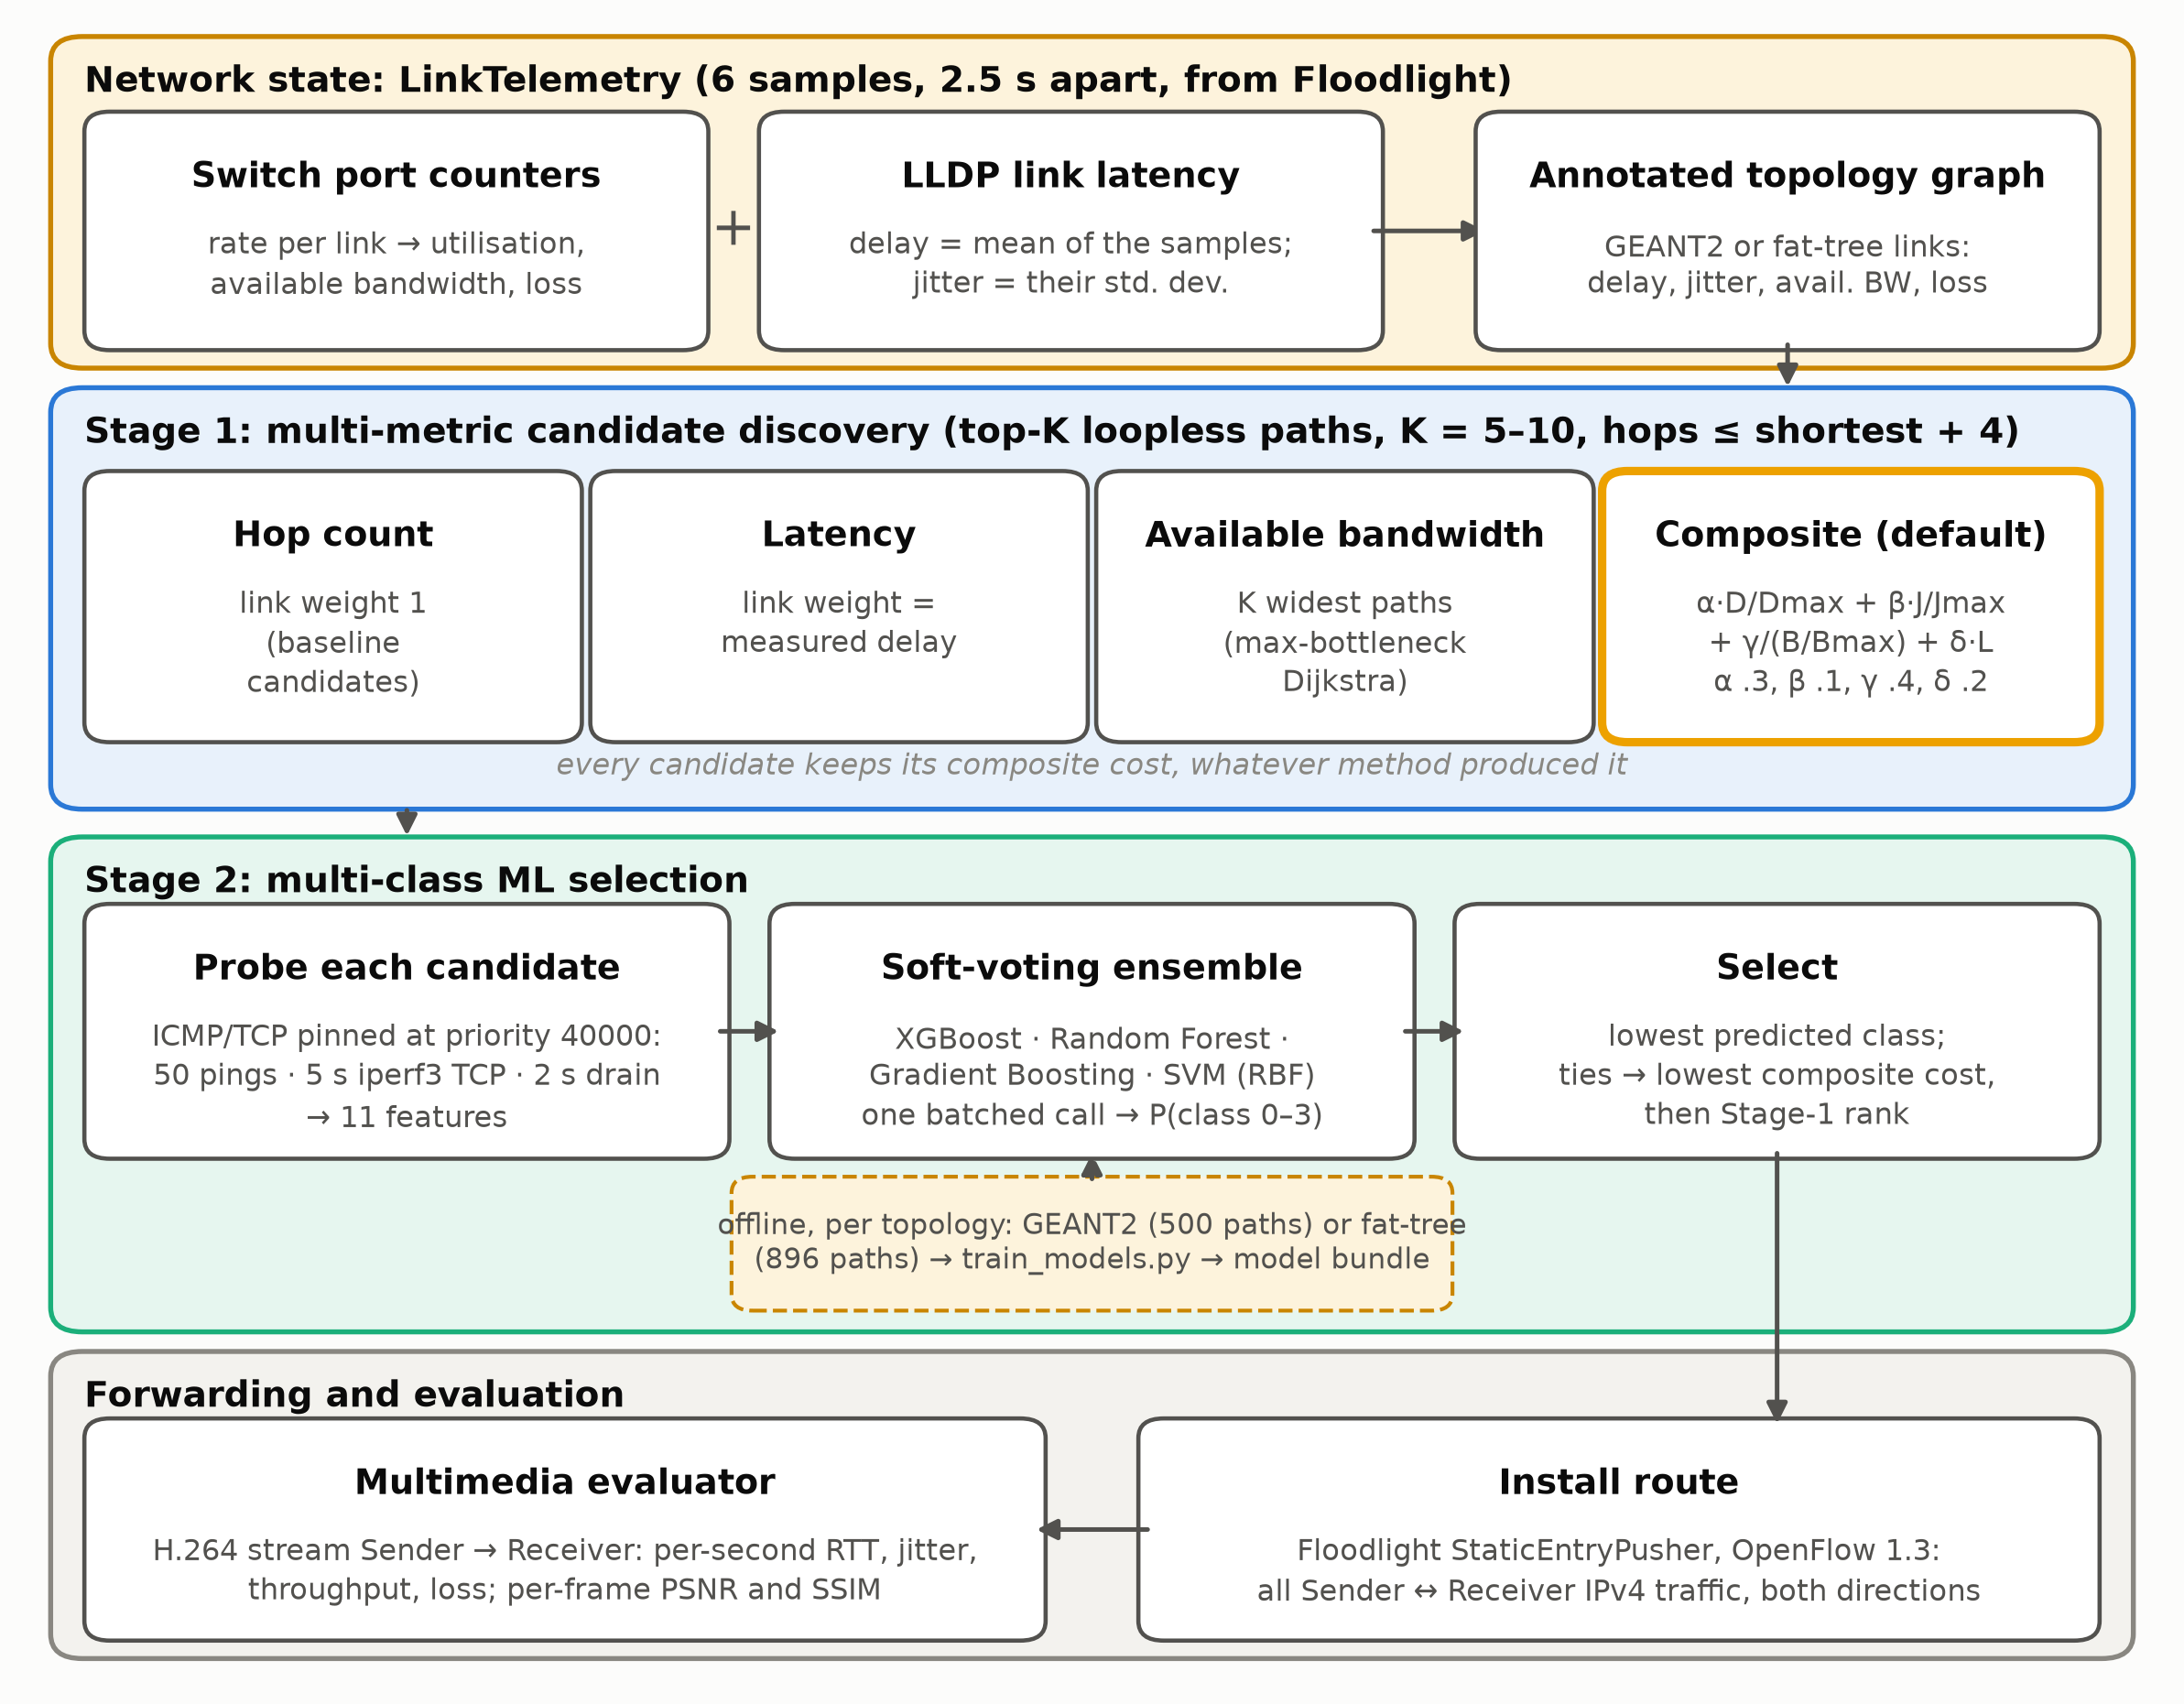
\includegraphics[width=0.82\textwidth]{pipeline.png}
\caption{Architecture of the proposed two-stage router. Link telemetry annotates the topology graph; Stage~1 returns
the top-$K$ candidates under one of four metrics (composite by default); Stage~2 probes the candidates, classifies
them in one batched ensemble call and selects the lowest class; the route is installed as static OpenFlow entries.}
\label{fig:pipeline}
\end{figure*}

\subsection{Architecture}
The system has five modules on top of Mininet~\cite{lantz2010mininet}, Open vSwitch~\cite{pfaff2015ovs} and the
Floodlight controller~\cite{floodlight}:
\begin{itemize}
\item \textbf{Topology and traffic.} Builds the emulated network and drives four-class background traffic: every
link carries one iperf3~\cite{iperf3} UDP flow per direction, pinned to that link, at a rate drawn from one of four
load bands (Extremely Low $<0.25$, Low $<0.5$, High $<0.8$, Extremely High $\le 1.2$ of capacity). A path's ground
truth is the class of its most loaded link.
\item \textbf{Telemetry.} Samples Floodlight six times, 2.5\,s apart, and derives per link the delay and jitter
(mean and standard deviation of LLDP latency), available bandwidth (capacity minus the busier direction's rate)
and loss (from port counters at both ends).
\item \textbf{Stage~1, path discovery.} Hop-bounded Yen's algorithm~\cite{yen1971kshortest} over hop count, delay,
widest path or the composite cost.
\item \textbf{Stage~2, selection.} Probing, feature extraction, the ensemble and the selection rule.
\item \textbf{Evaluation.} Streams the video, logs per-second QoS and scores per-frame quality.
\end{itemize}

\subsection{Proposed Algorithm}
\textit{Composite cost.} For link $uv$ with delay $D_{uv}$, jitter $J_{uv}$, available bandwidth $B_{uv}$ and loss
fraction $L_{uv}$, normalised by the maximum over all links,
\begin{equation}
c_{uv} = \alpha\frac{D_{uv}}{D_{\max}} + \beta\frac{J_{uv}}{J_{\max}} +
\frac{\gamma}{\max\!\left(B_{uv}/B_{\max},\,10^{-3}\right)} + \delta L_{uv},
\label{eq:cost}
\end{equation}
with $\alpha=0.3$, $\beta=0.1$, $\gamma=0.4$, $\delta=0.2$, the values used throughout the GEANT2 work. The
inverse-bandwidth term grows quickly as a link fills, so the cheapest paths avoid loaded links even when they are
longer. A path's cost is the sum of its link costs, and Yen's algorithm returns the five cheapest loopless paths of
at most the shortest hop distance plus four hops. Every candidate also carries its composite cost into Stage~2.

\textit{Features.} Each candidate is probed with its ICMP and TCP traffic pinned at higher priority than the route,
so probing never disturbs the video. The 11 features are the mean, minimum, maximum and deviation of RTT and the
loss of 50 pings; the throughput, bandwidth utilisation and retransmissions of a 5\,s iperf3 TCP test; the hop
count; and the maximum and mean link utilisation along the path from the telemetry snapshot.

\textit{Ensemble.} Four classifiers are trained per topology: XGBoost~\cite{chen2016xgboost}, Random
Forest~\cite{breiman2001rf}, Gradient Boosting~\cite{friedman2001gbm} and an RBF support vector
machine~\cite{cortes1995svm} with Platt-calibrated probabilities~\cite{platt1999probabilistic}. The deployed model
is their soft vote~\cite{kuncheva2004combining}: for a feature vector $\mathbf{x}$,
\begin{equation}
\hat{y}(\mathbf{x}) = \arg\max_{c\in\{0,1,2,3\}} \frac{1}{4}\sum_{m=1}^{4} P_m(c\mid\mathbf{x}).
\label{eq:vote}
\end{equation}

\textit{Selection.} The router installs the candidate with the lowest predicted class; ties go to the lower
composite cost and then to the earlier Stage~1 rank.

\subsection{Modifications to the Base Paper}
Table~\ref{tab:mods} lists what was changed, why, and how it addresses the limitations of Section~III.

\begin{table}[t]
\centering
\caption{Modifications to AIRSDN}
\label{tab:mods}
\footnotesize
\begin{tabularx}{\columnwidth}{@{}>{\raggedright\arraybackslash}p{1.45cm}LL@{}}
\toprule
Aspect & AIRSDN~\cite{ipek2025airsdn} & Proposed \\
\midrule
Candidates & 5 hop-count shortest paths & 5 cheapest paths under the composite cost~(\ref{eq:cost}); detours allowed up to +4 hops \\
Labels & 2 (low / high) & 4 (Extremely Low \ldots Extremely High) \\
Model & Logistic Regression & soft vote of XGBoost, RF, GB, SVM~(\ref{eq:vote}) \\
Inference & per candidate & one batched call for all $K$ \\
Features & 19 (incl.\ flow statistics) & 11 (ping, iperf3, hop count, link utilisation) \\
Tie-break & Stage~1 rank & composite cost, then rank \\
Topologies & NSFNET & GEANT2 and $k=4$ fat-tree, one model each \\
\bottomrule
\end{tabularx}
\end{table}

The composite candidates address limitation~1: a detour whose links are idle has a low cost even if it is longer,
so it enters the candidate set. Four classes address limitation~2 by ranking lightly loaded candidates. Batching
keeps the inference cost almost independent of $K$. Training one model per topology addresses limitation~3 without
asking a model to extrapolate to RTTs it never saw: the two topologies have different base delays.

\subsection{Step-by-Step Working Procedure}
\begin{enumerate}
\item \textbf{Offline.} Collect a labelled path dataset on the live emulated topology (Section~VI) and train the
four models and their ensemble.
\item \textbf{Telemetry.} When a flow arrives, take a link snapshot ($\approx$19\,s).
\item \textbf{Stage~1.} Annotate the graph and compute the top-5 composite-cost paths.
\item \textbf{Probe.} For each candidate, pin ICMP/TCP onto it, run 50 pings and a 5\,s iperf3 test, wait 2\,s
for the queues to drain, and remove the pin.
\item \textbf{Classify.} Stack the five feature vectors and call the ensemble once.
\item \textbf{Select and install.} Choose the lowest class and push static entries for all Sender--Receiver IPv4
traffic in both directions.
\end{enumerate}

\subsection{Algorithm}
\begin{algorithm}[t]
\caption{Two-stage multimedia route selection}
\label{alg:route}
\begin{algorithmic}[1]
\Require topology $G$, Sender $s$, Receiver $r$, $K$, weights $(\alpha,\beta,\gamma,\delta)$, ensemble $\mathcal{E}$
\State $T \gets$ \Call{LinkTelemetry}{} \Comment{delay, jitter, avail.\ BW, loss}
\State annotate every link $uv$ of $G$ with $c_{uv}$ from $T$ using (\ref{eq:cost})
\State $\mathcal{P} \gets$ \Call{Yen}{$G, s, r, K, c$, hops $\le d(s,r)+4$}
\For{each candidate $p_i \in \mathcal{P}$}
  \State pin ICMP/TCP of $(s,r)$ onto $p_i$
  \State $\mathbf{x}_i \gets$ \Call{Probe}{$p_i$} $\cup$ \Call{Util}{$T, p_i$} \Comment{11 features}
  \State remove the pin
\EndFor
\State $\mathbf{P} \gets \mathcal{E}.\Call{PredictProba}{[\mathbf{x}_1,\ldots,\mathbf{x}_K]}$ \Comment{one batched call}
\State $\hat{y}_i \gets \arg\max_c \mathbf{P}_{i,c}$
\State $p^\ast \gets \arg\min_i\,(\hat{y}_i,\ \mathrm{cost}(p_i),\ i)$
\State install $p^\ast$ for $(s,r)$ as static OpenFlow entries
\State \Return $p^\ast$
\end{algorithmic}
\end{algorithm}

Algorithm~\ref{alg:route} summarises the decision. Stage~1 costs $O(K\,n\,(m+n)\log n)$ for Yen's algorithm on a
graph with $n$ switches and $m$ links, which is milliseconds at this scale; the probes dominate the decision time.

% ---------------------------------------------------------------------------------------------------------
\section{Implementation and System Design}
\textit{Software and hardware.} The system runs on Ubuntu 24.04 (Linux 7.0) on a laptop with an AMD Ryzen~9 8945HS
(16 threads) and 14\,GB of RAM. The network is emulated with Mininet 2.3.1b4~\cite{lantz2010mininet} and Open
vSwitch 3.3~\cite{pfaff2015ovs} using OpenFlow~1.3~\cite{mckeown2008openflow}, under Floodlight 1.2 (master) on
Java~8~\cite{floodlight}. The code is Python 3.12 with NetworkX, scikit-learn 1.9~\cite{pedregosa2011sklearn} and
XGBoost 3.2~\cite{chen2016xgboost}. Traffic uses iperf3 3.16~\cite{iperf3}; the video is streamed and scored with
FFmpeg 6.1~\cite{ffmpeg}; datasets are profiled with ydata-profiling 4.18~\cite{ydataprofiling}.

\textit{Topologies.} Fig.~\ref{fig:topos} shows the two networks; Table~\ref{tab:topos} compares their structure.
GEANT2 uses the 24-node, 37-link edge list of RouteNet and DRL+GNN~\cite{rusek2020routenet,almasan2022drlgnn}; the
fat-tree is the standard $k=4$ design~\cite{alfares2008fattree} with 4 core, 8 aggregation and 8 edge switches.
Every switch-to-switch link is shaped to 10\,Mbit/s, 10\,ms one-way delay and a 1,000-packet queue in both
networks, so the topology is the only difference. Each switch has one host; on the fat-tree the hosts on core and
aggregation switches only source and sink background traffic.

\begin{figure*}[t]
\centering
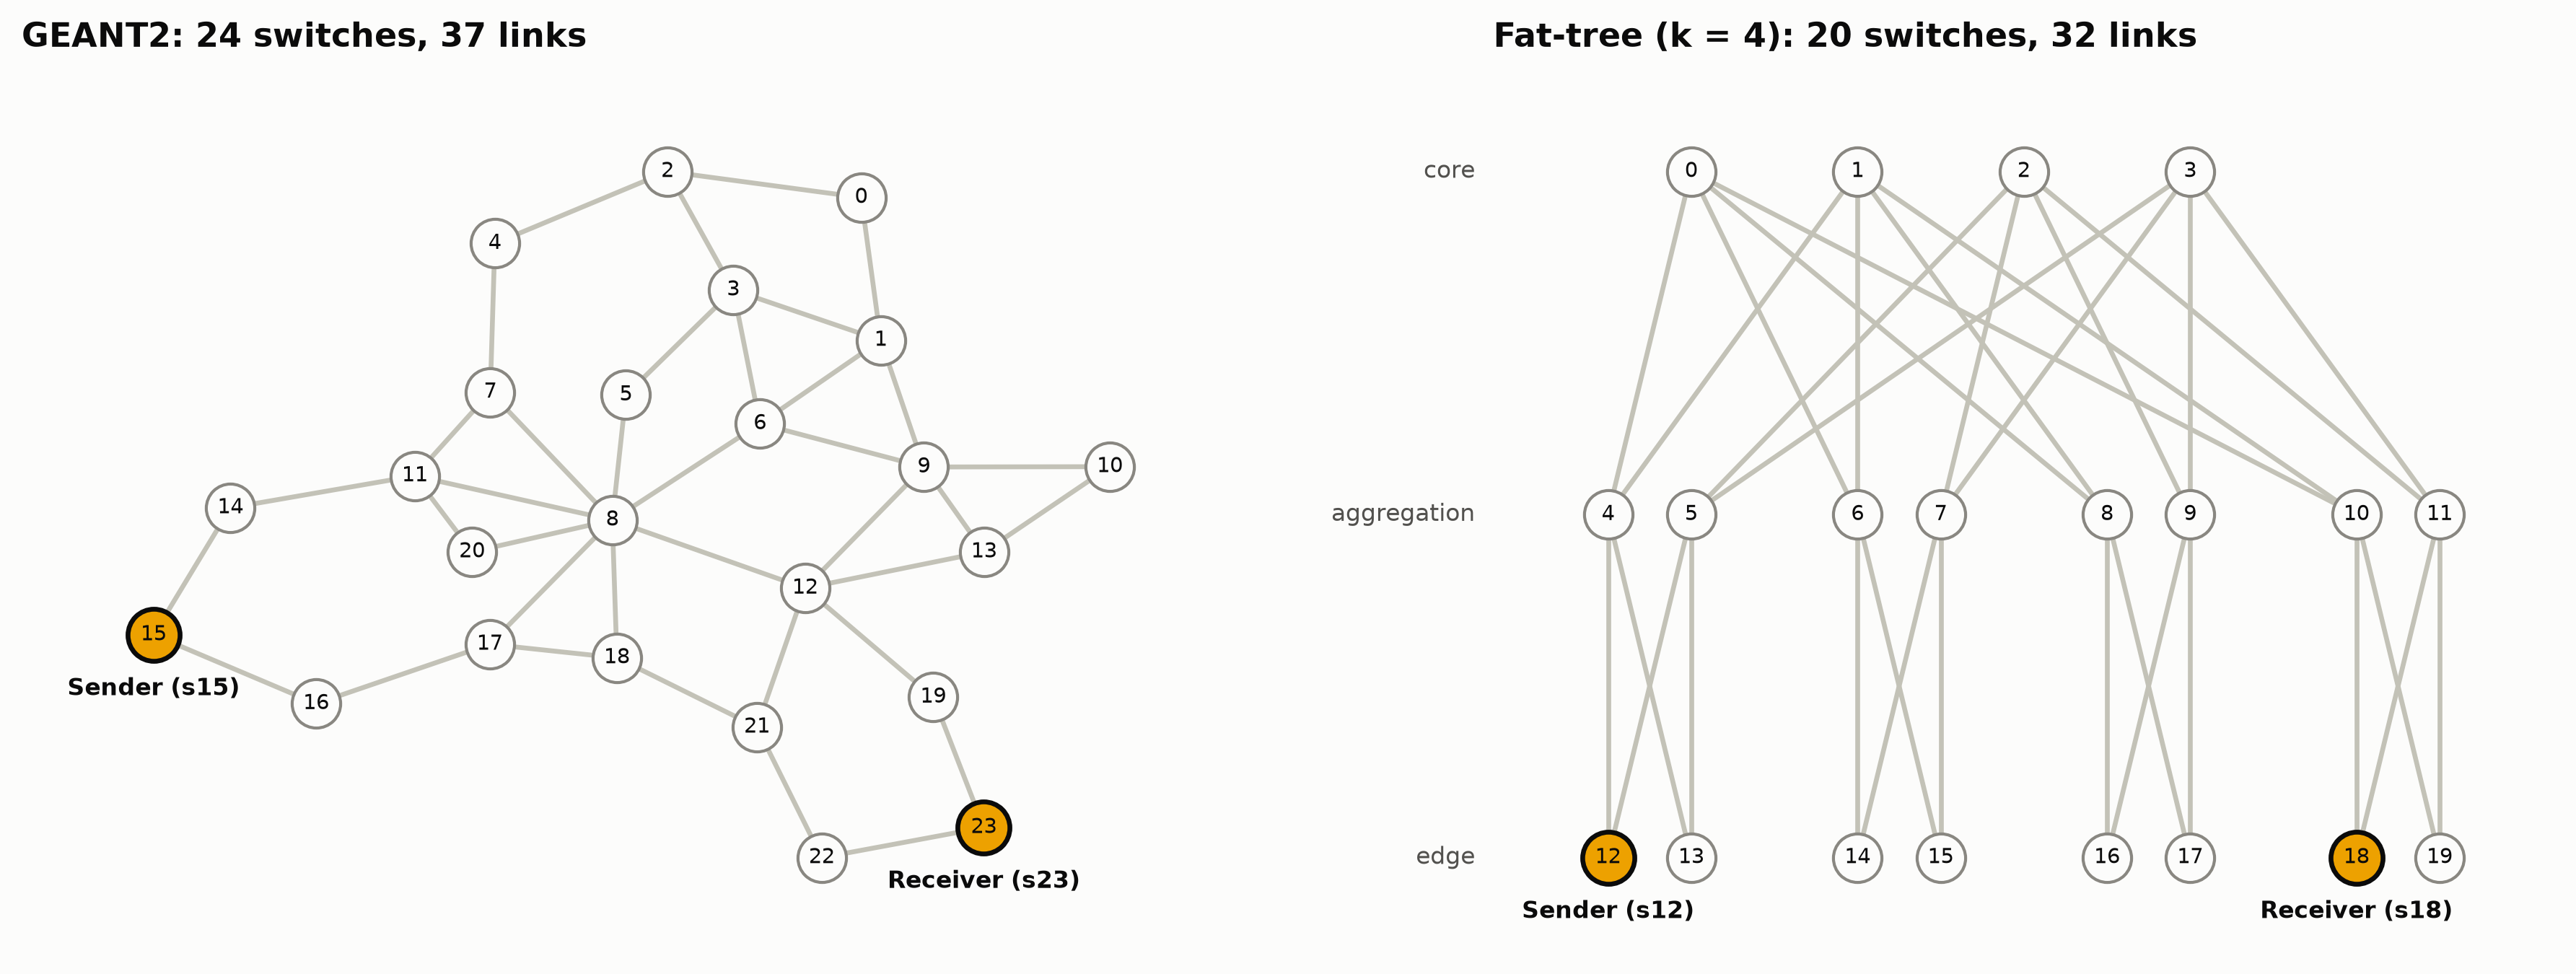
\includegraphics[width=0.86\textwidth]{topologies.png}
\caption{The two evaluation topologies with the video Sender and Receiver. GEANT2 is meshed with a hub (s8); the
fat-tree is layered, with four equal-cost 4-hop paths from s12 to s18, one through each core switch.}
\label{fig:topos}
\end{figure*}

\begin{table}[t]
\centering
\caption{Structural comparison of the topologies}
\label{tab:topos}
\footnotesize
\begin{tabular}{@{}lcc@{}}
\toprule
Property & GEANT2 & Fat-tree $k=4$ \\
\midrule
Switches / links & 24 / 37 & 20 / 32 \\
Degree & 2--8 (hub s8) & 4 core/agg., 2 edge \\
Diameter (hops) & 6 & 4 \\
Algebraic connectivity & 0.31 & 0.76 \\
Max.\ betweenness centrality & 0.52 & 0.14 \\
Sender $\rightarrow$ Receiver & s15 $\rightarrow$ s23 & s12 $\rightarrow$ s18 \\
Hop-count candidates (hops) & 6, 6, 6, 7, 7 & 4, 4, 4, 4, 6 \\
\bottomrule
\end{tabular}
\end{table}

\textit{Datasets.} Each dataset was collected on its live emulated topology. In every epoch the traffic generator
applies a new four-class load scenario, the collector probes the Sender--Receiver candidates and three random host
pairs with the same 11-feature probe, and labels each path with the generator's ground-truth bottleneck class,
never with a measured value. Classes are capped at a quarter of the target so the datasets are balanced: GEANT2 has
500 paths (125 per class, 65 epochs) and the fat-tree 896 paths (224 per class, 114 epochs, trimmed by seeded
random sampling from 912 rows).

\textit{Important parameters.} $K=5$; hop bound shortest $+4$; weights $(0.3, 0.1, 0.4, 0.2)$; telemetry 6
samples at 2.5\,s; 50 pings at 50\,ms; 5\,s iperf3 TCP; 2\,s drain; data split 70/15/15, stratified, seed 40;
Random Forest 300 trees; XGBoost with early stopping on the validation split.

\textit{Workflow.} The modules run in order from one script: train each topology's ensemble, run an offline compute
benchmark, run the live benchmark on GEANT2 and then on the fat-tree, and assemble every figure with the data it
was drawn from.

% ---------------------------------------------------------------------------------------------------------
\section{Results and Discussion}
\subsection{Experimental Setup and Evaluation Metrics}
Each topology was evaluated in five seeded scenarios (seeds 1000--1004). In each scenario every link's load is
drawn from the four-class model and every link of the hop-count shortest path is then forced to Extremely High,
the situation that motivates load-aware routing. Five methods run one after another on the same scenario and the
same 66\,s H.264 video (1920$\times$1048, 60\,fps, 4,007 frames, about 4.7\,Mbit/s):
\begin{itemize}
\item \textbf{Hop-count:} shortest path ($K=1$).
\item \textbf{Latency:} lowest measured delay ($K=1$).
\item \textbf{Bandwidth:} widest path on measured available bandwidth ($K=1$).
\item \textbf{Baseline (hop-count + ML):} AIRSDN's candidate strategy, five hop-count paths, scored by the same
four-class ensemble as the proposed method, so that only Stage~1 differs.
\item \textbf{Proposed (combined + ML):} composite top-5 and the ensemble.
\end{itemize}
The metrics are the mean per-second video throughput, the whole-stream video packet loss and the per-second loss of
a 200\,kbit/s UDP probe, the mean RTT of one ping per second, RFC~3550 jitter~\cite{rfc3550} of the probe, the
FFmpeg PSNR and SSIM~\cite{wang2004ssim} of the received video, the ground-truth class of the chosen path, and the
time of every decision step.

\subsection{Results of the Base Paper / Baseline}
The base paper was first reproduced on its own NSFNET scenario with its binary Logistic Regression model. The
reproduction chose the same path as the paper's Fig.~15 and measured 351\,ms mean RTT, 6.52\,Mbit/s and
38.1\,dB PSNR (SSIM 0.997), close to the reported 354\,ms and 37.3\,dB; hop-count routing measured 1,830\,ms and
20.4\,dB against the reported 2,063\,ms and 21.5\,dB. In the two-topology evaluation the baseline is the
AIRSDN-style selector with the four-class ensemble, which is a stronger baseline than binary Logistic Regression.

\textit{Datasets and models.} Profiling found no missing values or duplicate rows in either dataset.
Fig.~\ref{fig:hist} shows that throughput and maximum link utilisation spread across their whole range while RTT is
nearly constant except for the Extremely High class: background traffic below capacity builds no queue. The median
RTT of the three lower classes is 120.2--120.3\,ms on GEANT2 and 80.3--86.5\,ms on the fat-tree, but rises to
about 2.4\,s in the Extremely High class, and ping loss is zero in 84--85\,\% of rows. The correlation matrices
(Fig.~\ref{fig:corr}) confirm that the class follows throughput and maximum link utilisation (0.88--0.95) far more
than RTT (0.42--0.46). Hop count correlates with RTT at 0.71 on GEANT2 but only 0.05 on the fat-tree, where 75\,\%
of paths have the same length, so the fat-tree model cannot lean on path length.

\begin{figure*}[t]
\centering
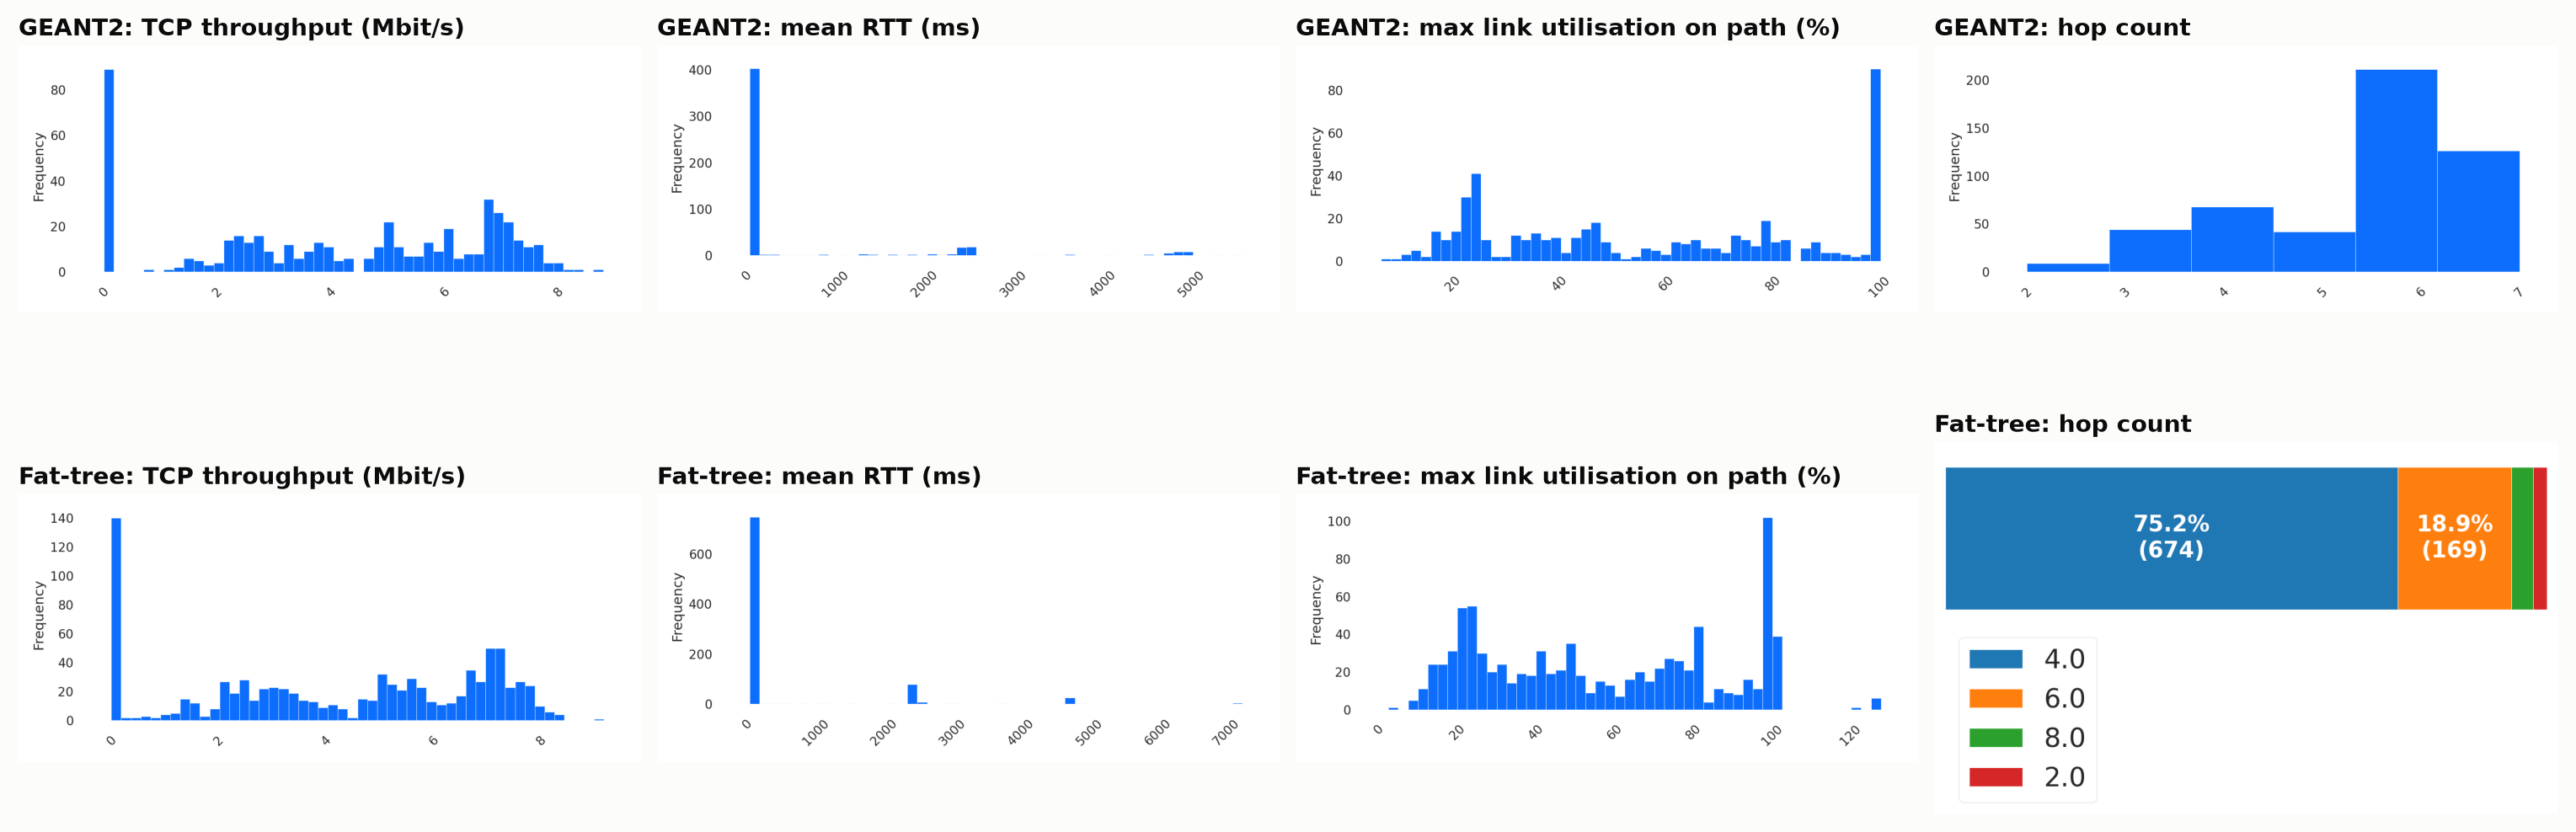
\includegraphics[width=\textwidth]{profile_histograms.png}
\caption{Feature distributions from the ydata-profiling reports of the two datasets. The fat-tree hop count has
only four values and is profiled as a categorical variable.}
\label{fig:hist}
\end{figure*}

\begin{figure*}[t]
\centering
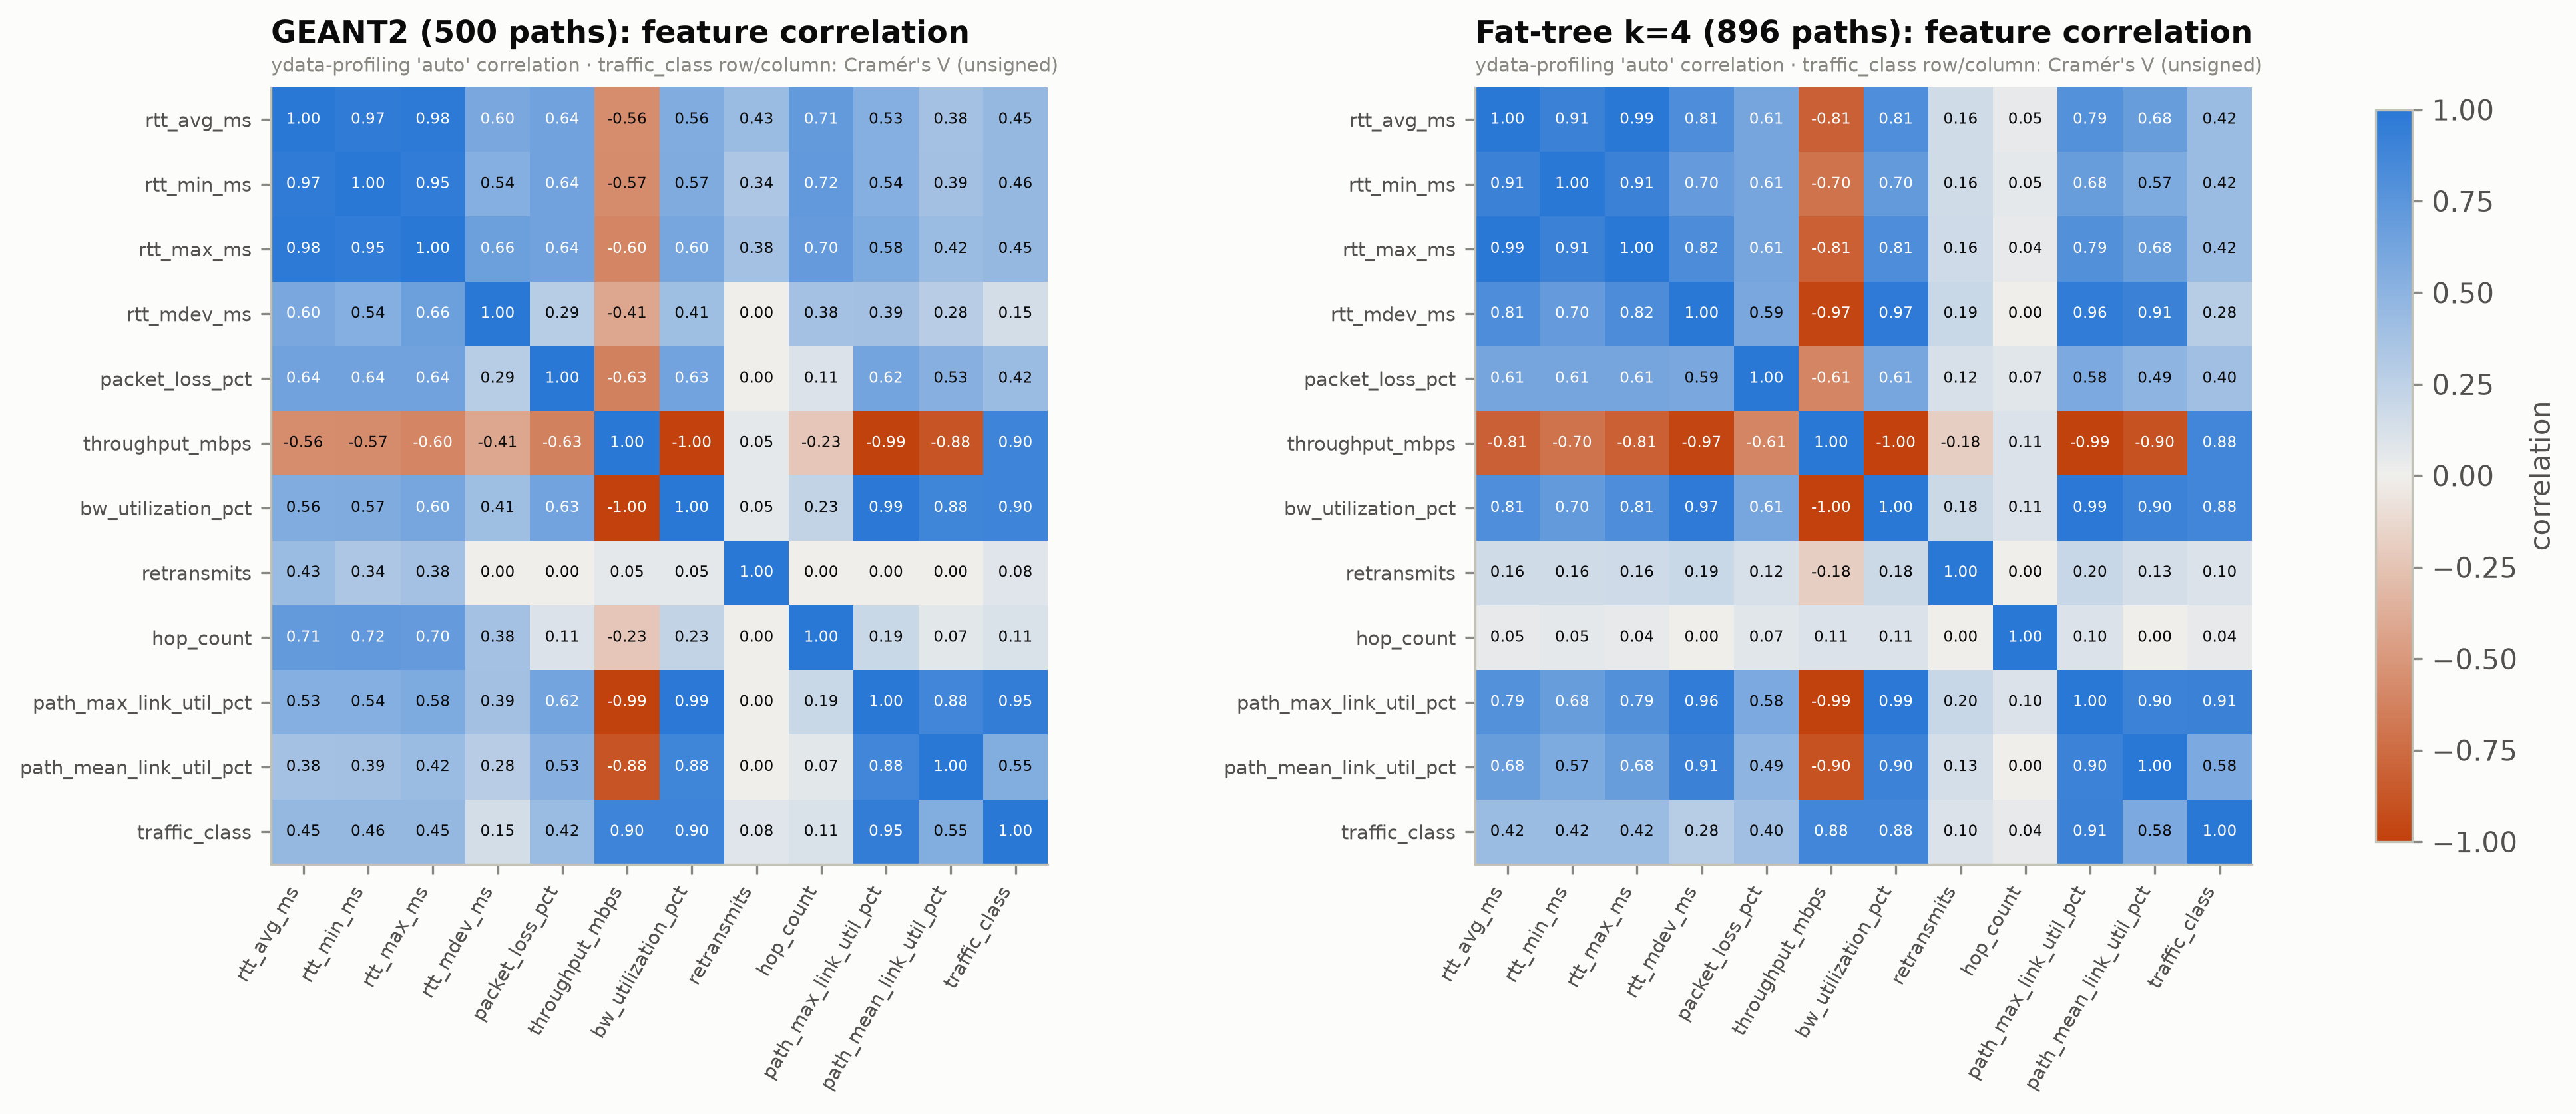
\includegraphics[width=0.92\textwidth]{correlation.png}
\caption{Feature correlation from the profiling reports (ydata-profiling ``auto'' correlation; the class row and
column use Cram\'er's V and are unsigned).}
\label{fig:corr}
\end{figure*}

Table~\ref{tab:models} lists the test scores. Both ensembles exceed the 95\,\% objective. On GEANT2 the ensemble
misclassifies two of 75 test paths; on the fat-tree it misclassifies two Low paths as Extremely Low out of 135
(Fig.~\ref{fig:confusion}). Live, the ensembles classified 47 of 50 (GEANT2) and 48 of 50 (fat-tree) probed
candidates correctly.

\begin{table}[t]
\centering
\caption{Test-set scores (macro averages)}
\label{tab:models}
\footnotesize
\setlength{\tabcolsep}{3.4pt}
\begin{tabular}{@{}lcccc@{}}
\toprule
& \multicolumn{2}{c}{GEANT2 (75 paths)} & \multicolumn{2}{c}{Fat-tree (135 paths)} \\
Model & Acc. & F1 & Acc. & F1 \\
\midrule
XGBoost & 0.973 & 0.974 & 0.985 & 0.985 \\
Random Forest & 0.973 & 0.974 & 0.993 & 0.993 \\
Gradient Boosting & 0.973 & 0.974 & 0.985 & 0.985 \\
SVM (RBF) & 0.933 & 0.931 & 0.926 & 0.926 \\
\textbf{Soft-voting ensemble} & \textbf{0.973} & \textbf{0.974} & \textbf{0.985} & \textbf{0.985} \\
\bottomrule
\end{tabular}
\end{table}

\begin{figure}[t]
\centering
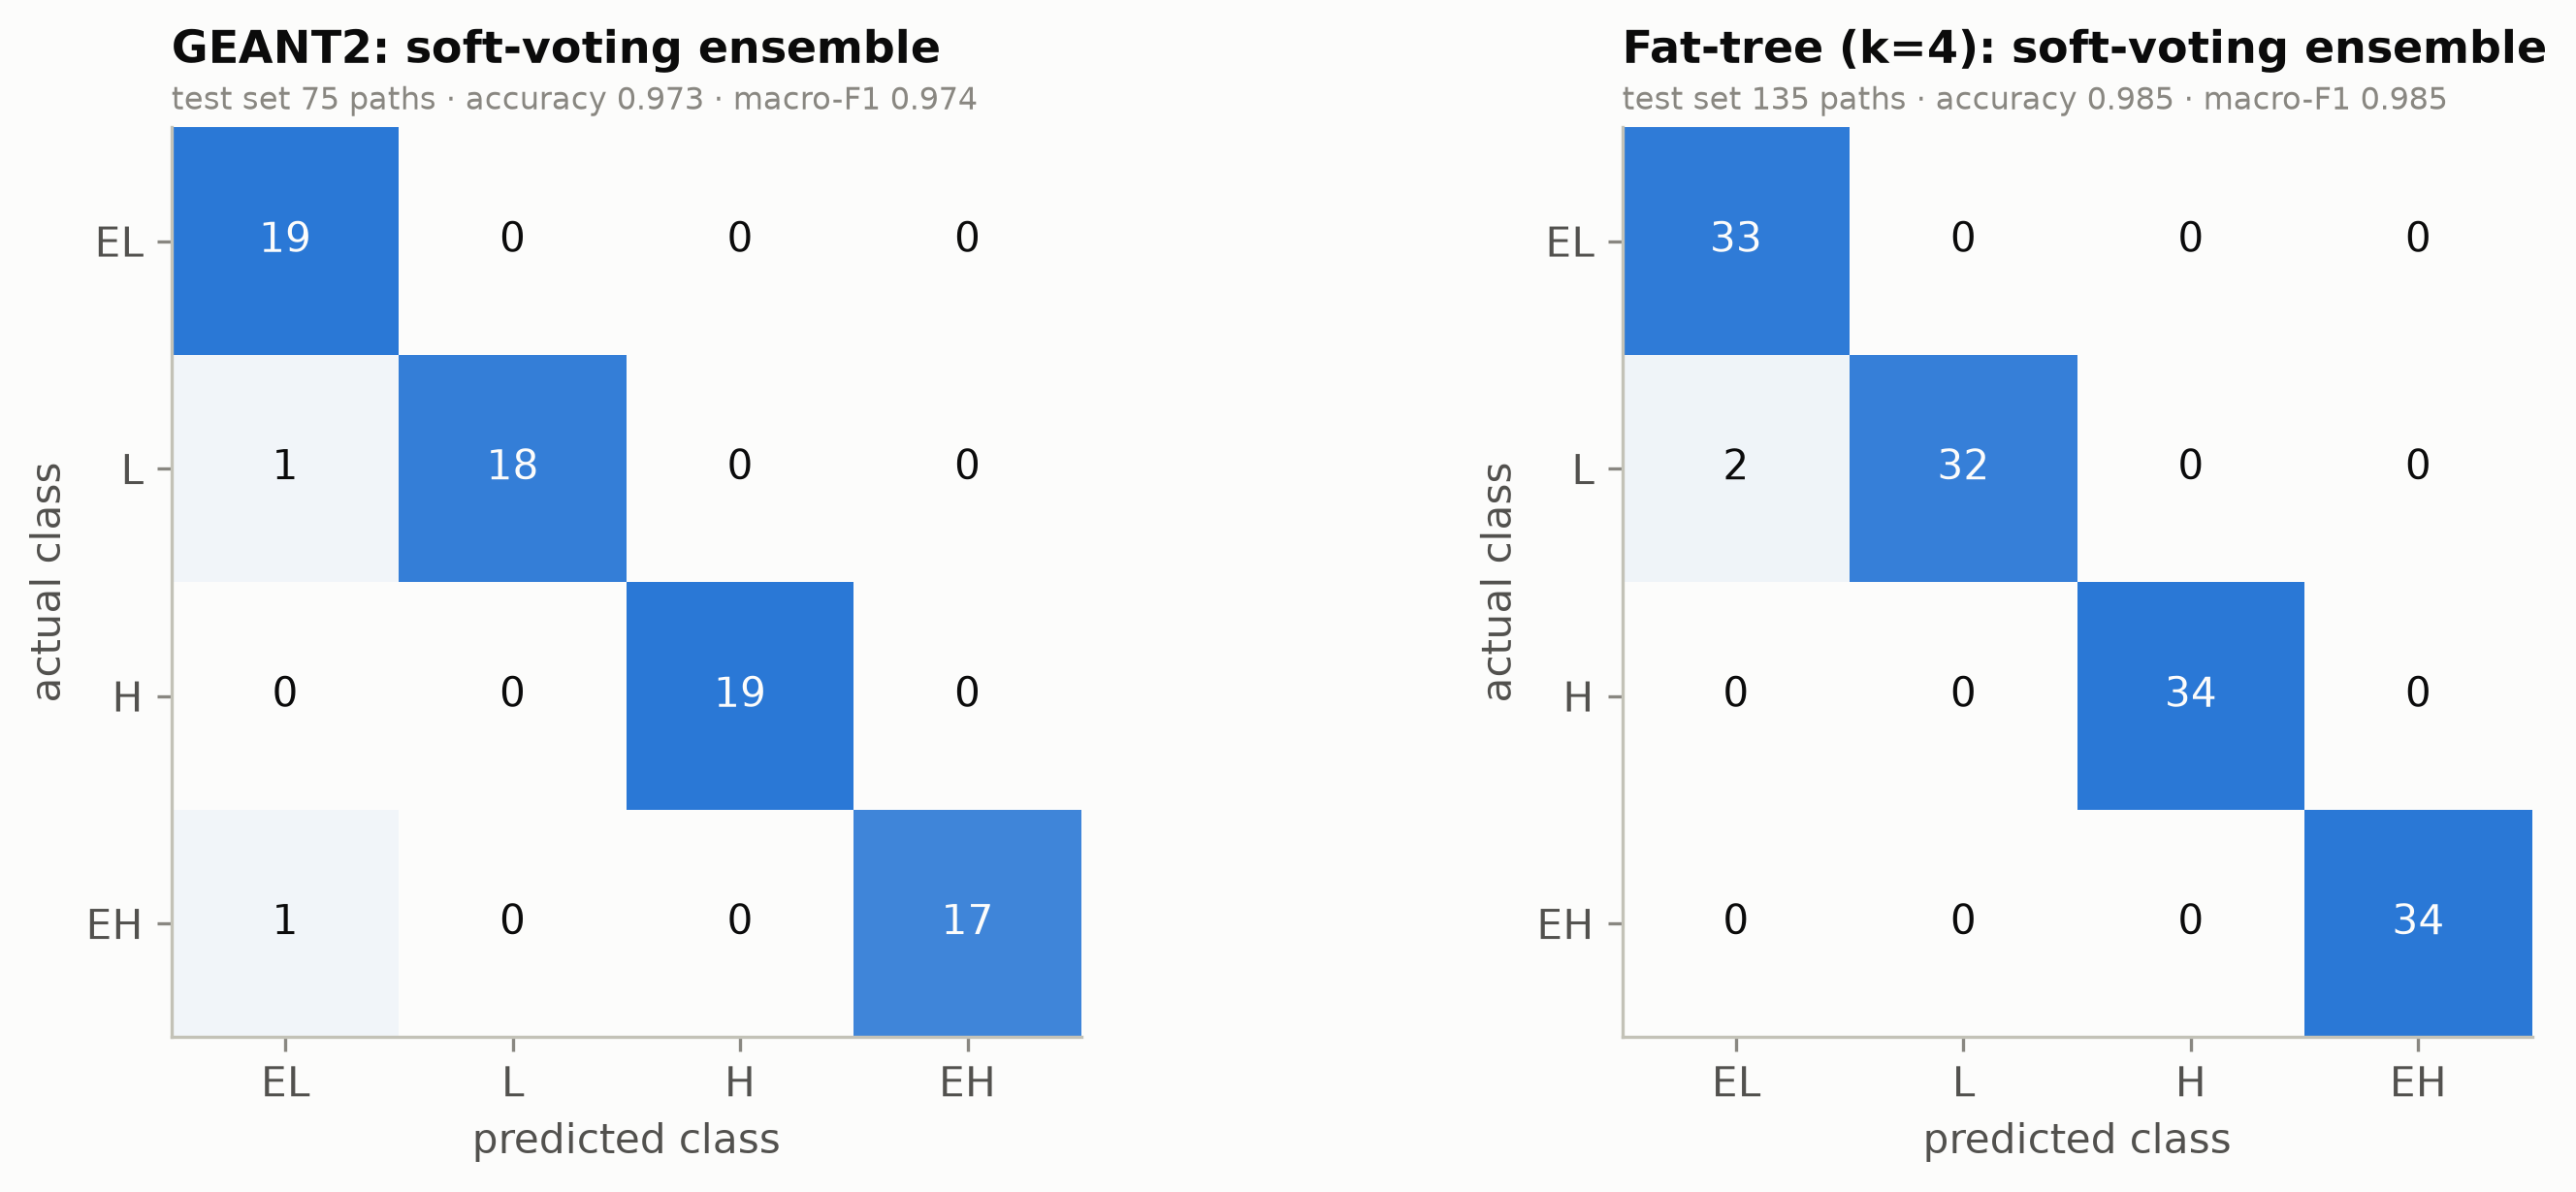
\includegraphics[width=\columnwidth]{confusion.png}
\caption{Confusion matrices of the two ensembles on their test sets.}
\label{fig:confusion}
\end{figure}

\subsection{Results of the Proposed Method}
Table~\ref{tab:results} gives the mean of each metric over the five scenarios. On GEANT2 the proposed method
delivered the video without loss in all five scenarios, at 38.43\,dB PSNR, 0.998 SSIM, 4.62\,Mbit/s and 157\,ms
mean RTT, and every path it chose was the least-congested path reachable within the hop bound (Table~\ref{tab:oracle}).

\begin{table*}[t]
\centering
\caption{Mean results over five scenarios per topology (whole-stream video loss; RTT n/a where every echo was lost)}
\label{tab:results}
\footnotesize
\setlength{\tabcolsep}{3.4pt}
\begin{tabular}{@{}l ccccccc ccccccc@{}}
\toprule
& \multicolumn{7}{c}{GEANT2} & \multicolumn{7}{c}{Fat-tree ($k=4$)} \\
\cmidrule(lr){2-8}\cmidrule(l){9-15}
Method & Thr. & Loss & RTT & Jitter & PSNR & SSIM & Class & Thr. & Loss & RTT & Jitter & PSNR & SSIM & Class \\
& Mbit/s & \% & ms & ms & dB & & 0--3 & Mbit/s & \% & ms & ms & dB & & 0--3 \\
\midrule
Hop-count & 0.76 & 82.6 & 13,064 & 17.0 & 14.8 & 0.739 & 3.00 & 0.96 & 78.3 & 8,607 & 10.4 & 14.9 & 0.746 & 3.00 \\
Latency & 4.50 & 2.3 & 530 & 14.2 & 31.3 & 0.949 & 1.00 & 4.21 & 8.2 & 1,019 & 13.9 & 29.4 & 0.902 & 1.40 \\
Bandwidth & 4.61 & 0.0 & 169 & 13.3 & 38.4 & 0.998 & 0.20 & 4.30 & 6.6 & 798 & 13.9 & 29.4 & 0.901 & 1.40 \\
Baseline (hop + ML) & 4.50 & 2.1 & 532 & 14.3 & 31.4 & 0.950 & 1.00 & 4.33 & 5.9 & 793 & 13.2 & 29.5 & 0.903 & 1.40 \\
\textbf{Proposed} & \textbf{4.62} & \textbf{0.0} & \textbf{157} & \textbf{13.2} & \textbf{38.4} & \textbf{0.998} & \textbf{0.20} & 4.31 & 6.6 & 792 & 13.3 & 29.2 & 0.893 & 1.40 \\
\bottomrule
\end{tabular}
\end{table*}

\begin{table}[t]
\centering
\caption{Ground-truth class of the chosen path per scenario, and the best class reachable within the hop bound}
\label{tab:oracle}
\footnotesize
\setlength{\tabcolsep}{3.4pt}
\begin{tabular}{@{}lccccc ccccc@{}}
\toprule
& \multicolumn{5}{c}{GEANT2} & \multicolumn{5}{c}{Fat-tree} \\
\cmidrule(lr){2-6}\cmidrule(l){7-11}
Scenario & 0 & 1 & 2 & 3 & 4 & 0 & 1 & 2 & 3 & 4 \\
\midrule
Best reachable & 0 & 1 & 0 & 0 & 0 & 3 & 0 & 0 & 3 & 1 \\
\midrule
Hop-count & 3 & 3 & 3 & 3 & 3 & 3 & 3 & 3 & 3 & 3 \\
Latency & 2 & 1 & 0 & 2 & 0 & 3 & 0 & 0 & 3 & 1 \\
Bandwidth & 0 & 1 & 0 & 0 & 0 & 3 & 0 & 0 & 3 & 1 \\
Baseline & 2 & 1 & 0 & 2 & 0 & 3 & 0 & 0 & 3 & 1 \\
\textbf{Proposed} & \textbf{0} & \textbf{1} & \textbf{0} & \textbf{0} & \textbf{0} & 3 & 0 & 0 & 3 & 1 \\
\bottomrule
\end{tabular}
\end{table}

Fig.~\ref{fig:paths} shows why. In GEANT2 scenario~0 the forced congestion covers s15--s14--s11--s8--s12--s19--s23,
and the other short paths cross a High link (s17--s18). All five hop-count candidates therefore have a High or
Extremely High bottleneck, and the baseline correctly chose the best of them, a 6-hop High path. The composite cost
penalised the loaded links and offered a 7-hop detour, s15--s16--s17--s8--s18--s21--s22--s23, whose links are all
Extremely Low; the ensemble classified it as such and chose it. The same happened in scenario~3. In scenarios 1, 2
and 4 the baseline's candidates already contained the best path and both methods chose it.

\begin{figure*}[t]
\centering
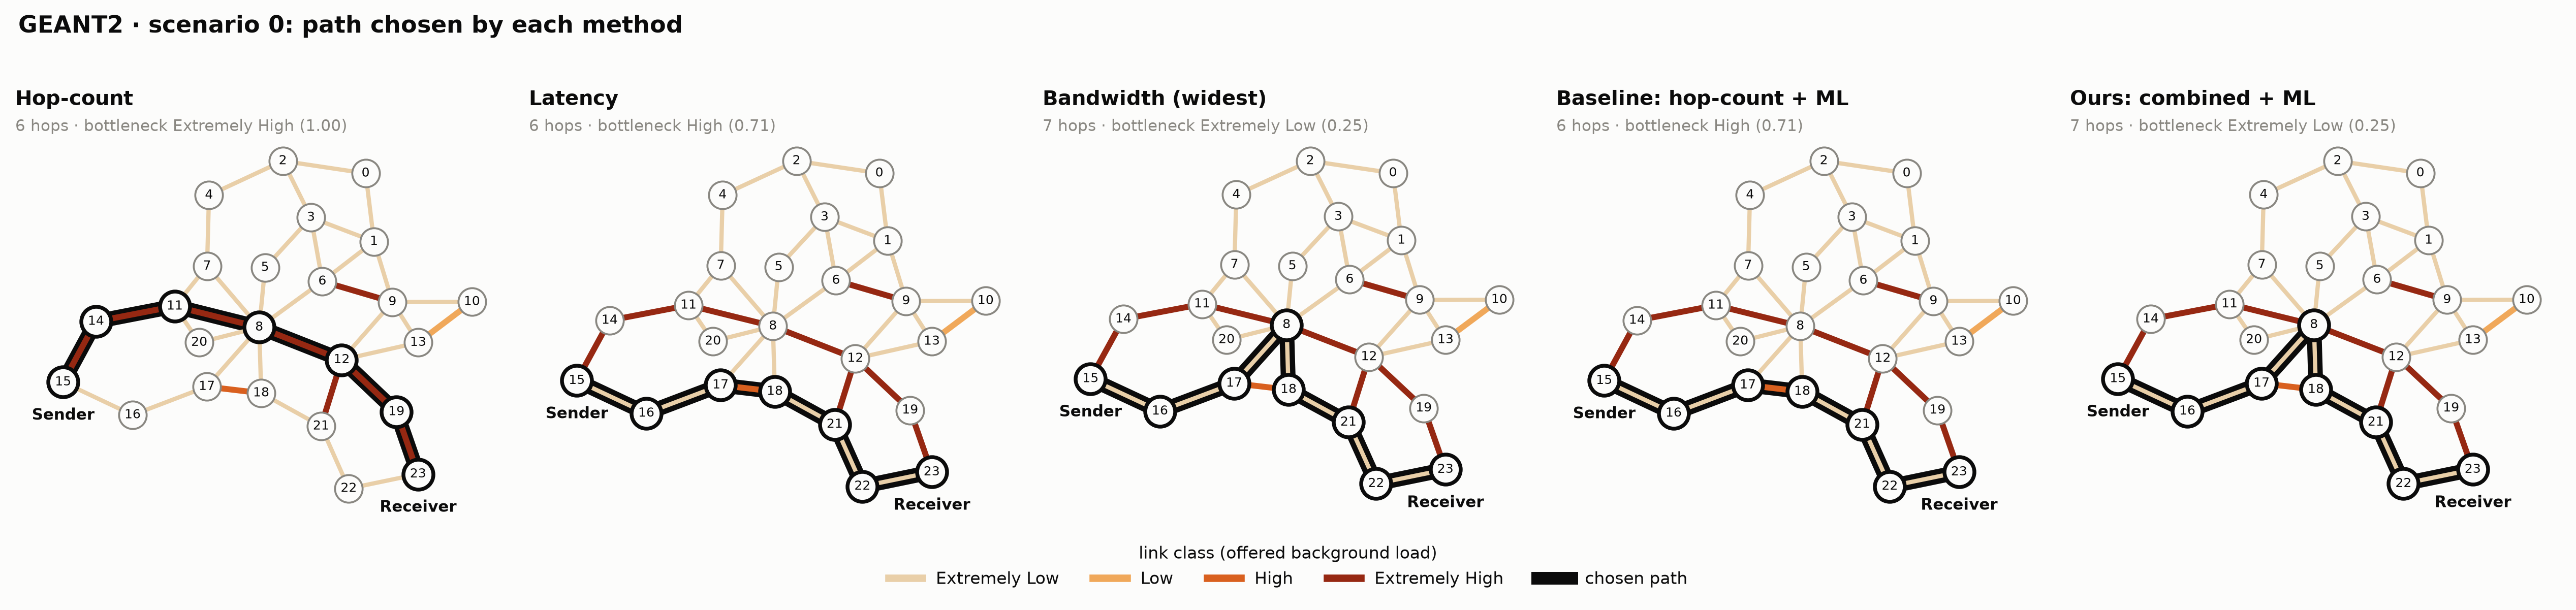
\includegraphics[width=\textwidth]{paths_geant2_s0.png}
\caption{Paths chosen in GEANT2 scenario~0, drawn over the offered-load class of every link. Only bandwidth routing
and the proposed method leave the High and Extremely High region.}
\label{fig:paths}
\end{figure*}

The per-second traces (Fig.~\ref{fig:ts}, left) show the consequence for the video: on the 6-hop High path, the
baseline and latency routing hold an RTT of about 1.3\,s for most of the transfer as the queue fills, while the
proposed method stays near 150\,ms; hop-count routing loses most echoes and its RTT exceeds 10\,s.

\begin{figure*}[t]
\centering
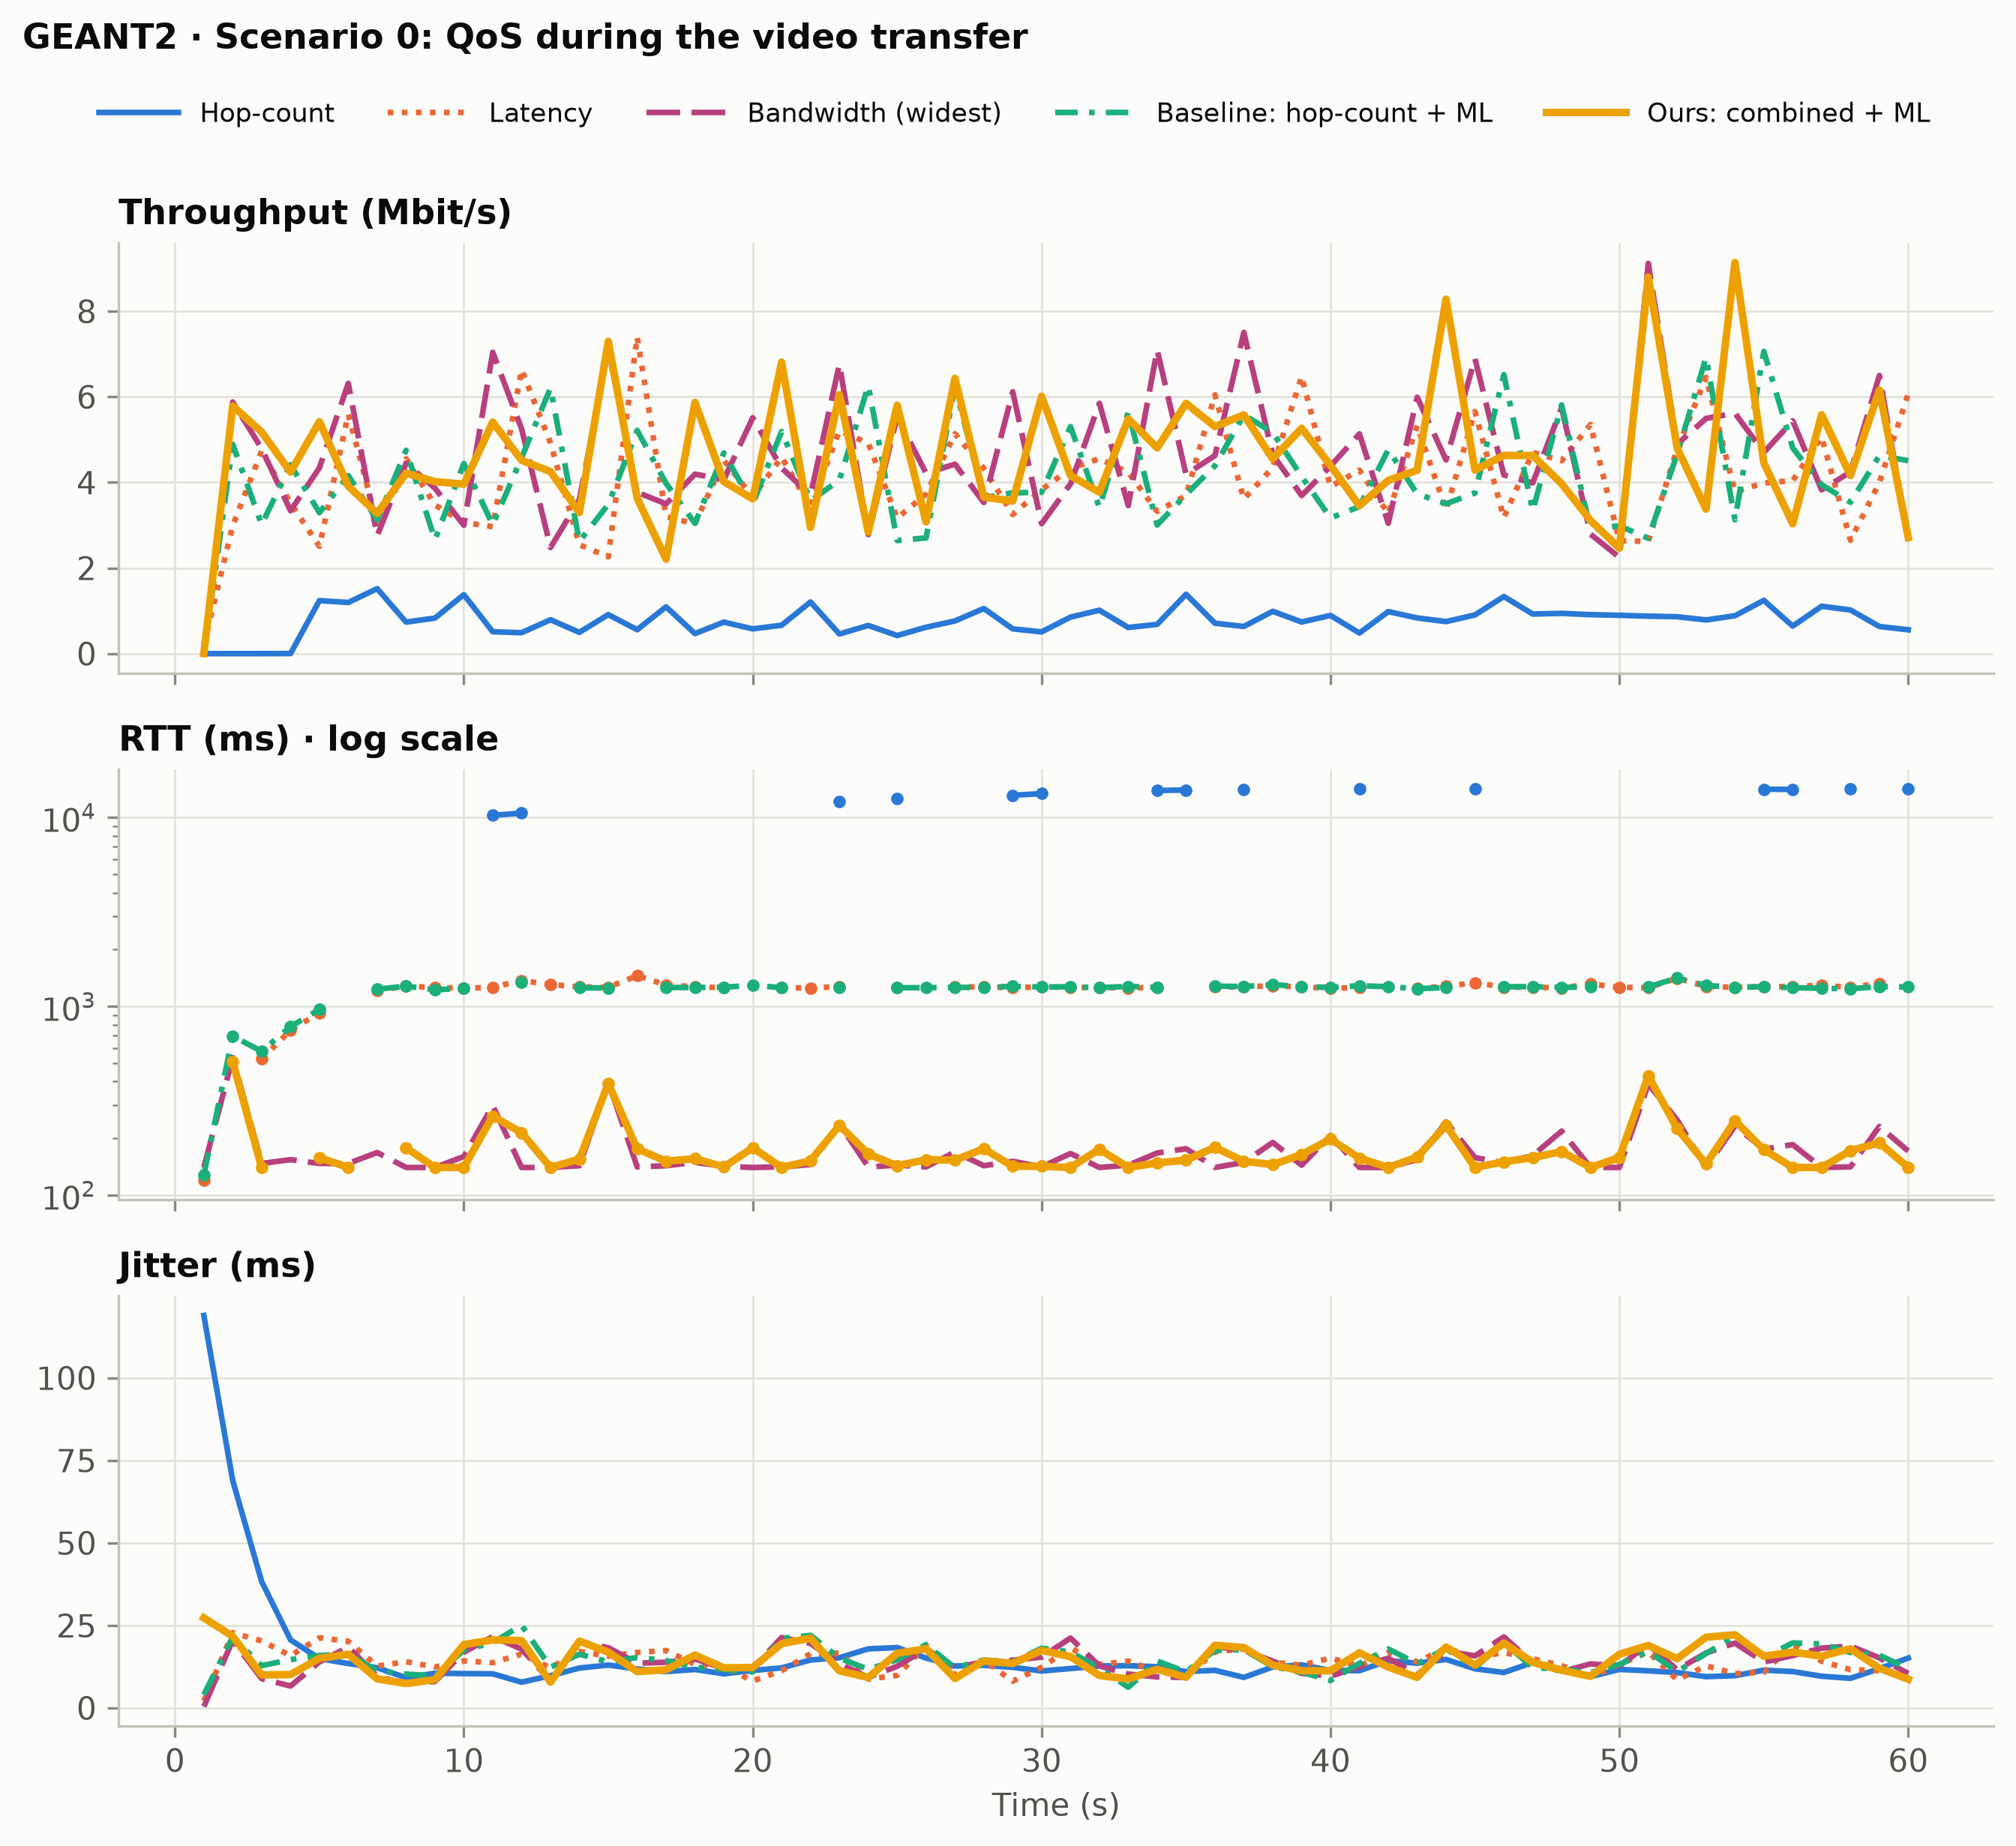
\includegraphics[width=0.49\textwidth]{ts_geant2_s0.png}\hfill
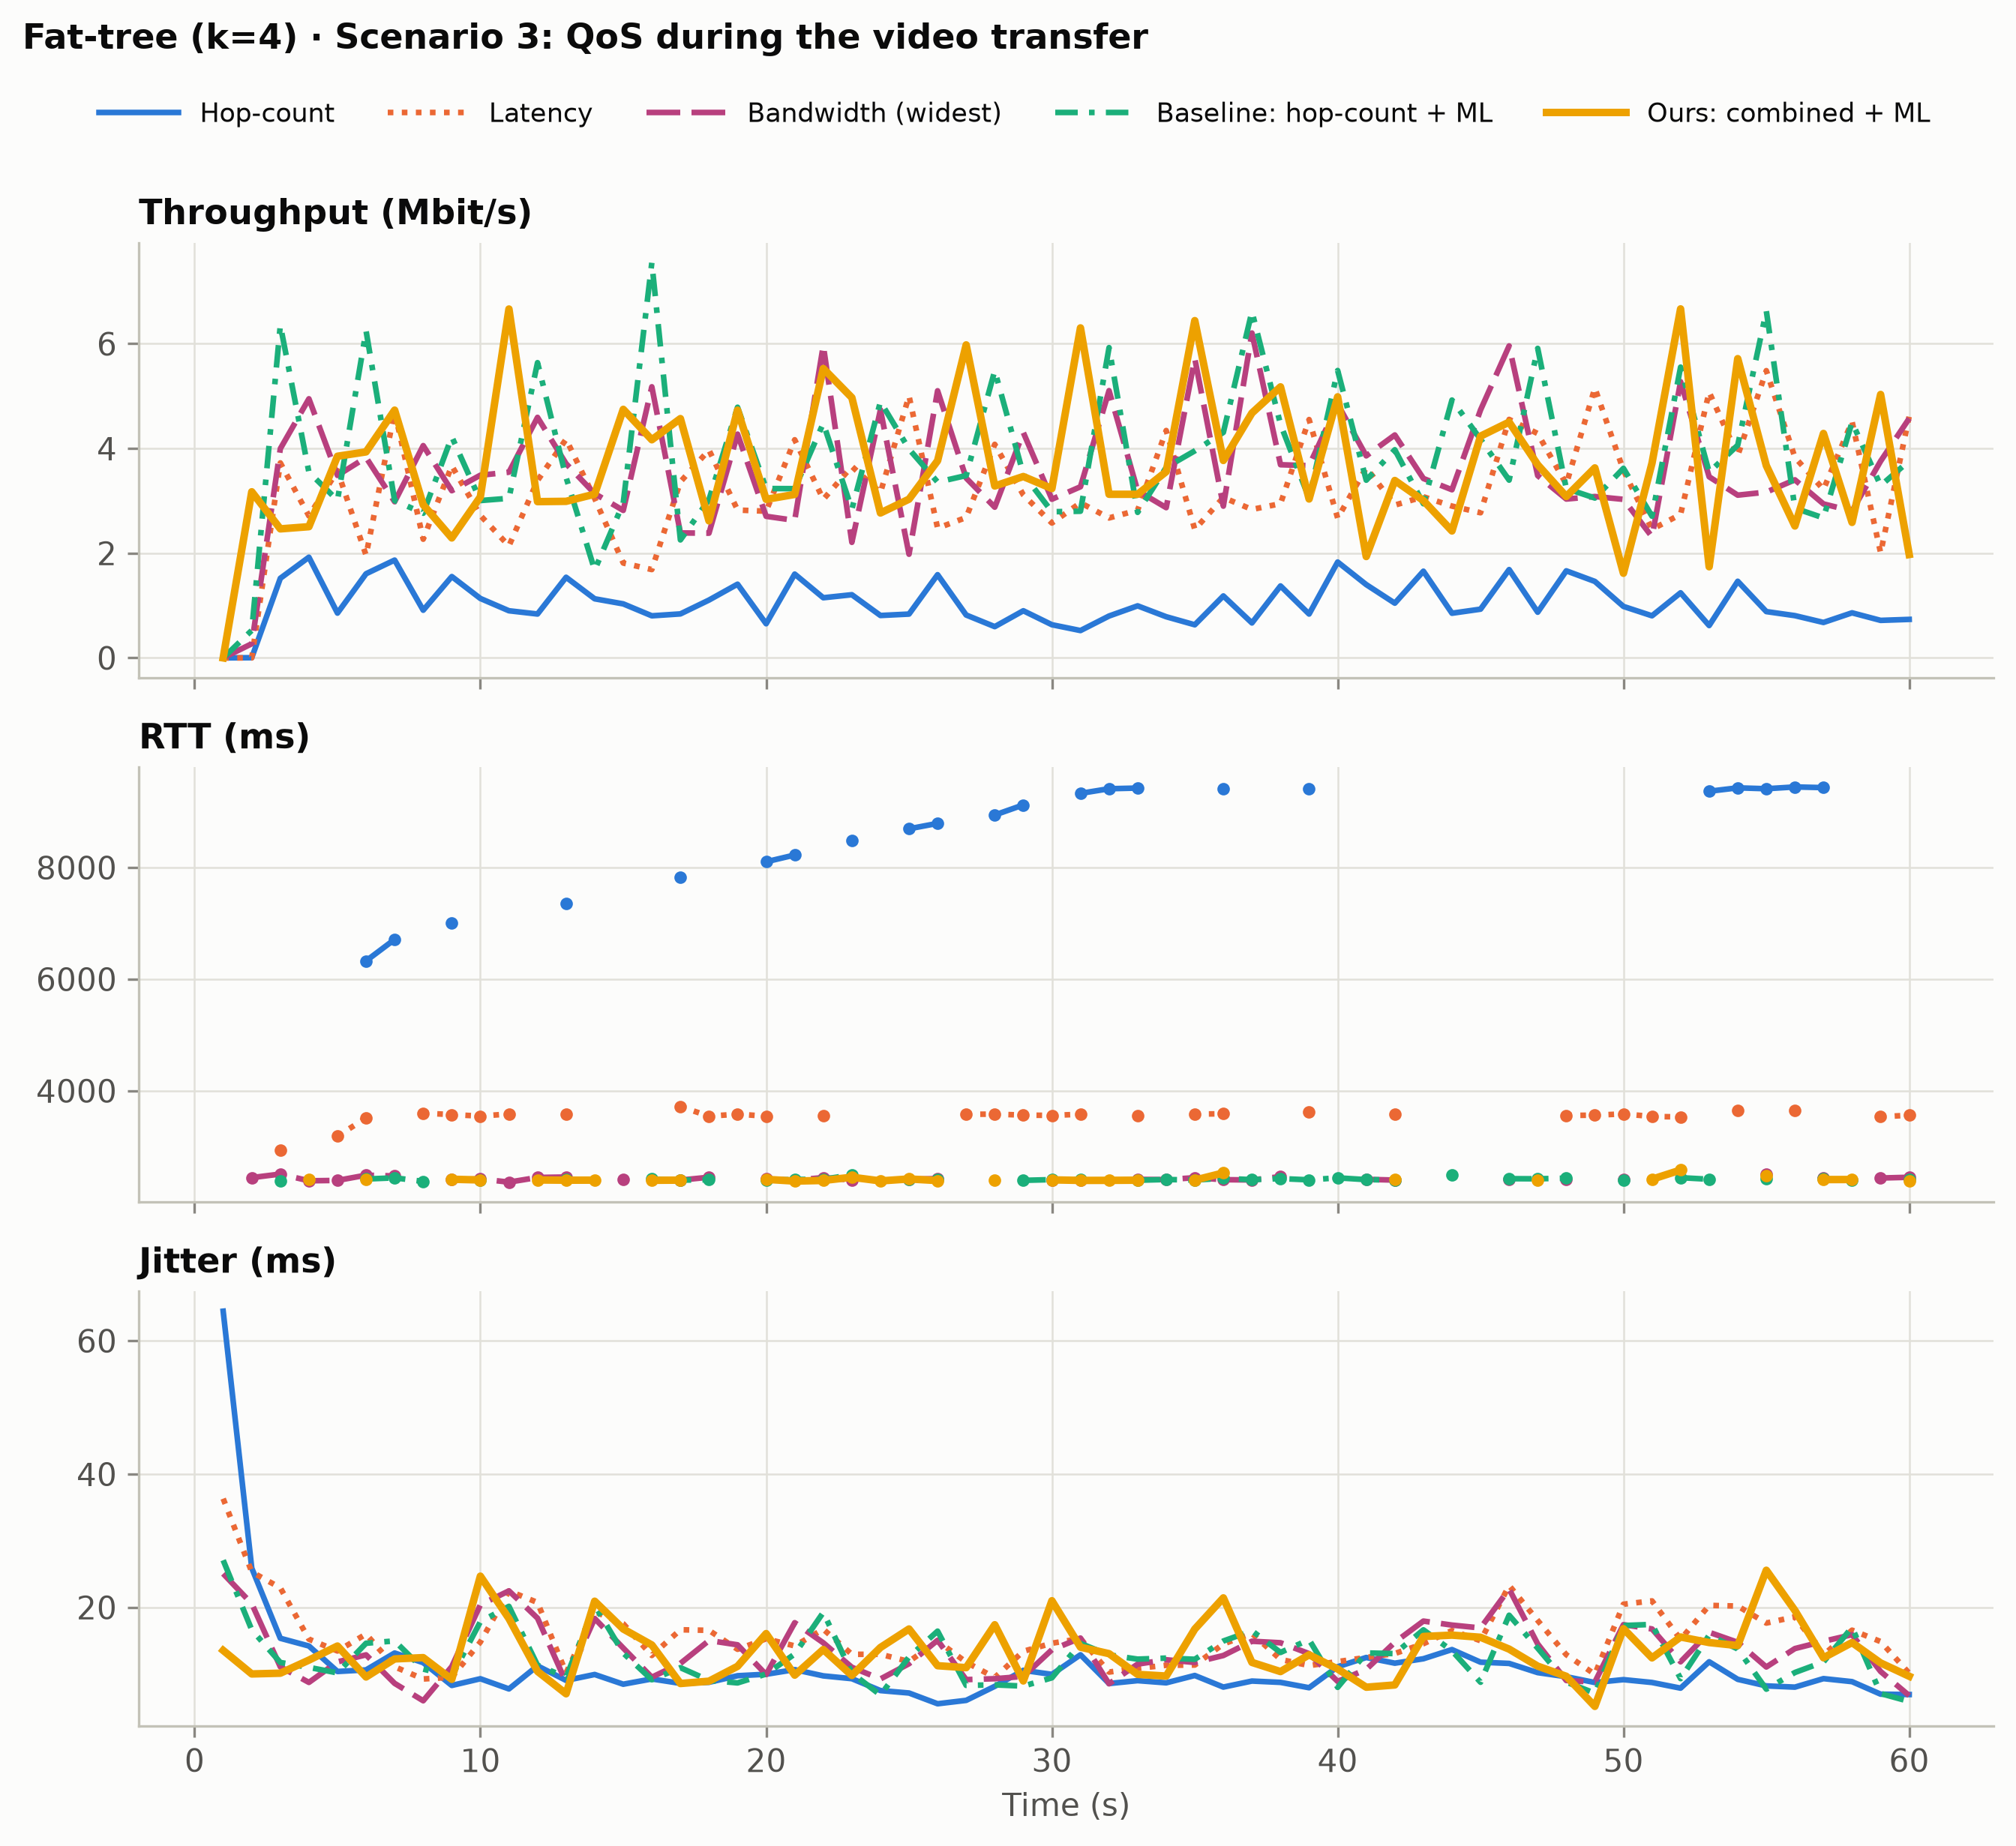
\includegraphics[width=0.49\textwidth]{ts_fattree_s3.png}
\caption{Per-second video throughput, RTT (log scale) and jitter. Left: GEANT2 scenario~0. Right: fat-tree
scenario~3, where every path within the hop bound crosses an Extremely High link.}
\label{fig:ts}
\end{figure*}

\subsection{Comparative Analysis}
Fig.~\ref{fig:qos} compares the five methods on both topologies, and Fig.~\ref{fig:overview}
summarises every decision.

\begin{figure*}[t]
\centering
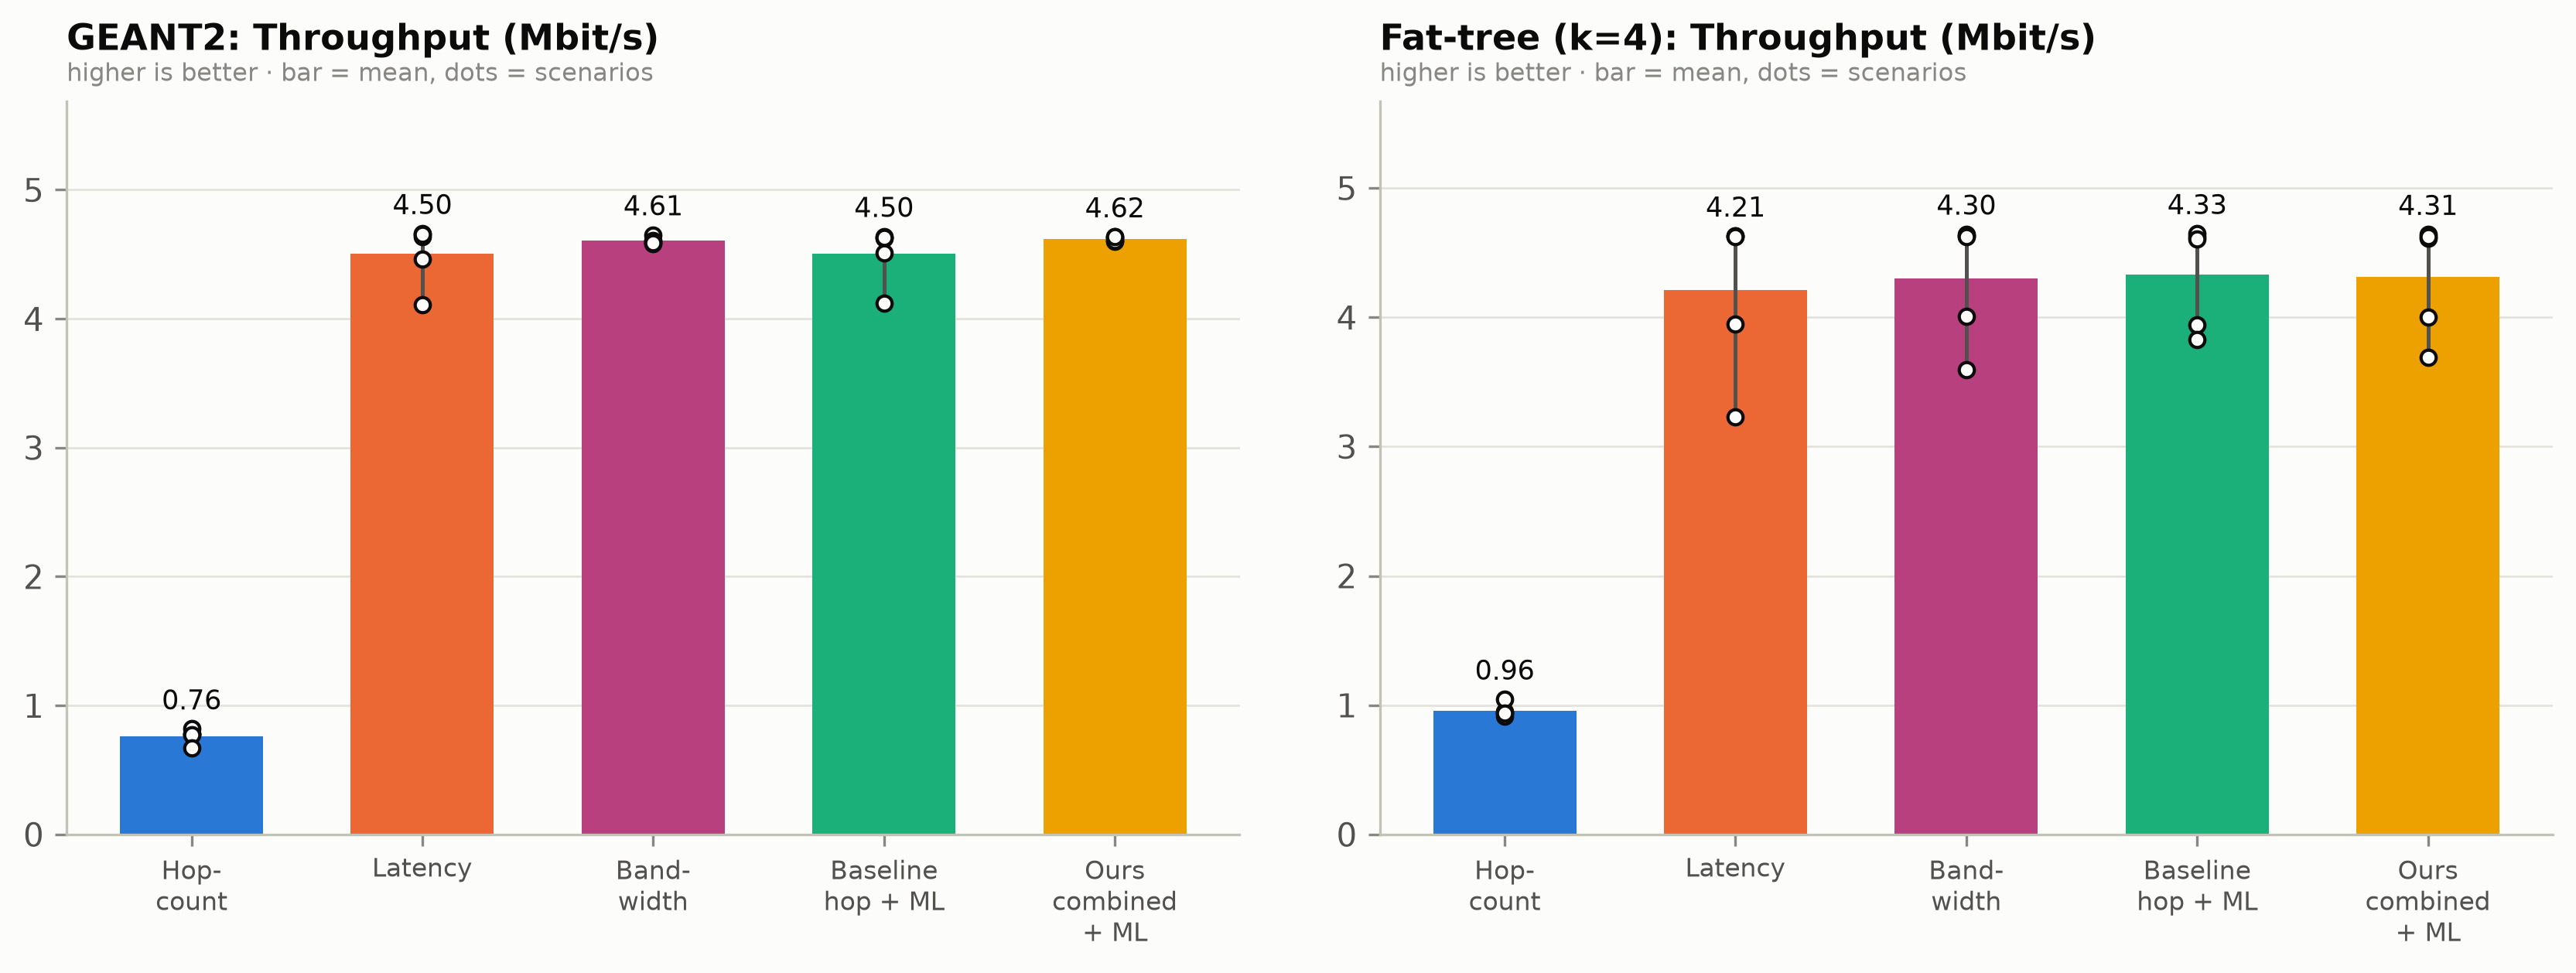
\includegraphics[width=0.49\textwidth]{throughput.png}\hfill
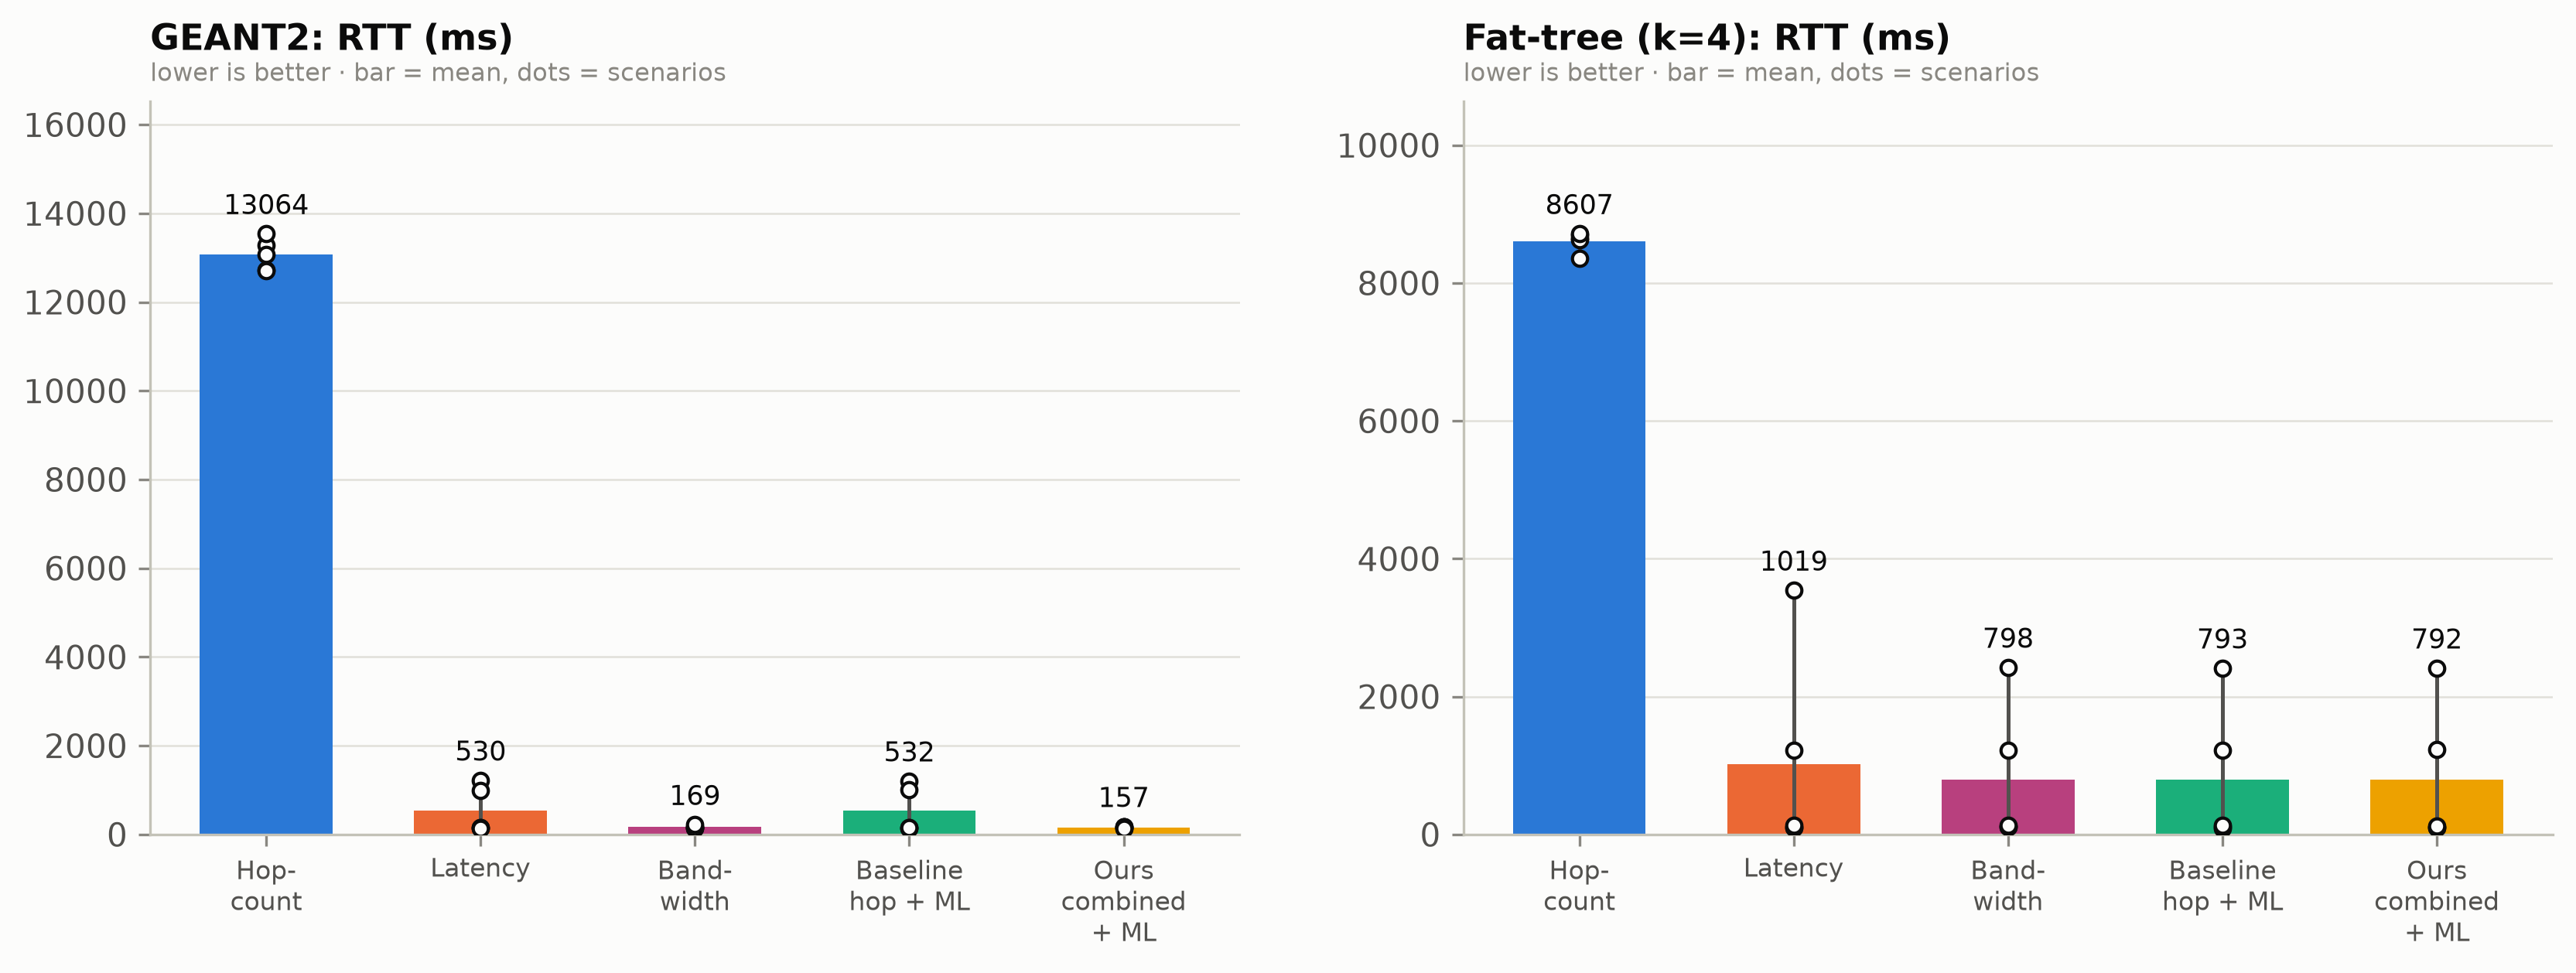
\includegraphics[width=0.49\textwidth]{rtt.png}\\[2pt]
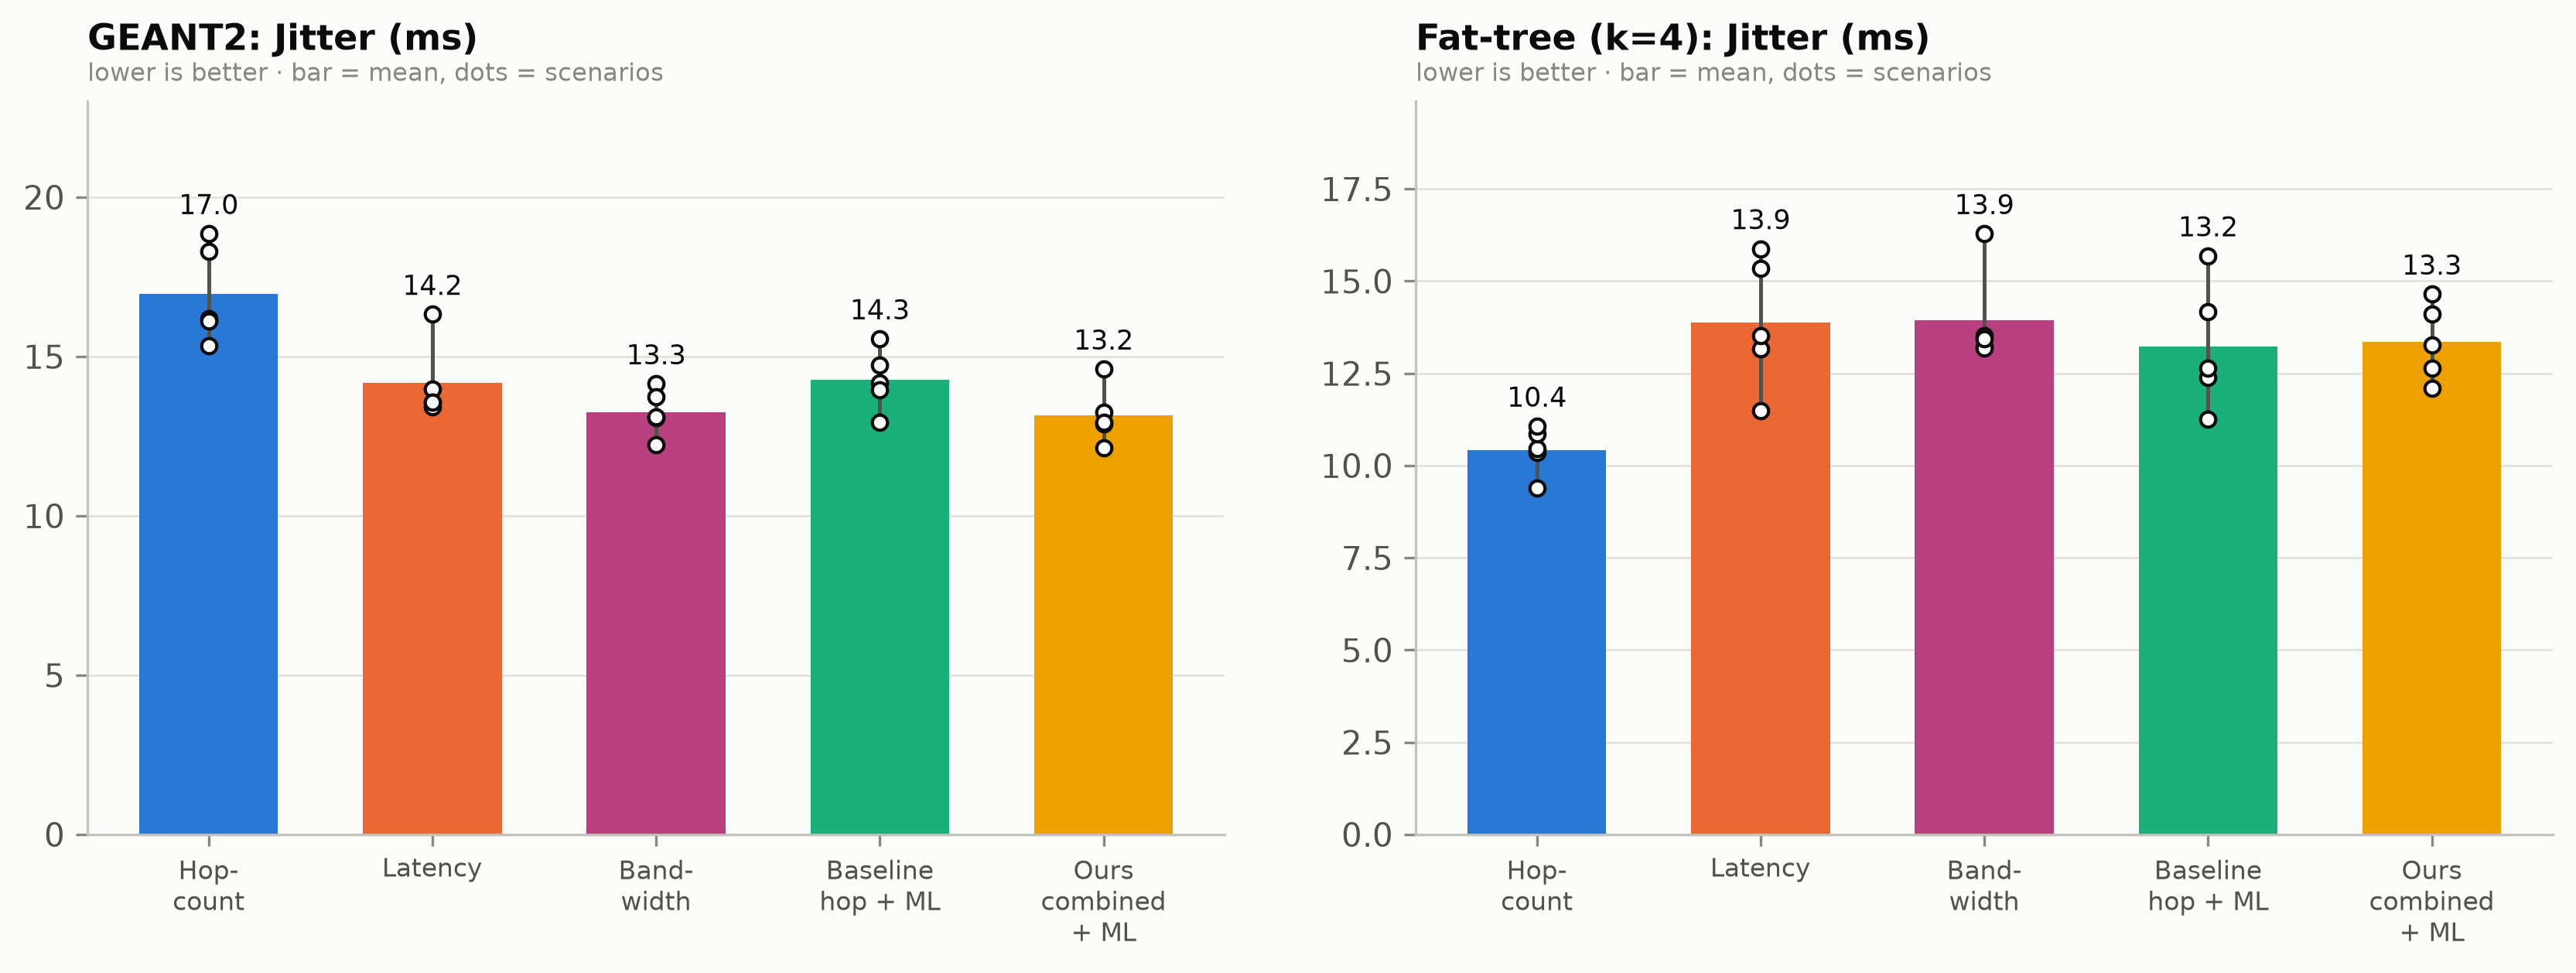
\includegraphics[width=0.49\textwidth]{jitter.png}\hfill
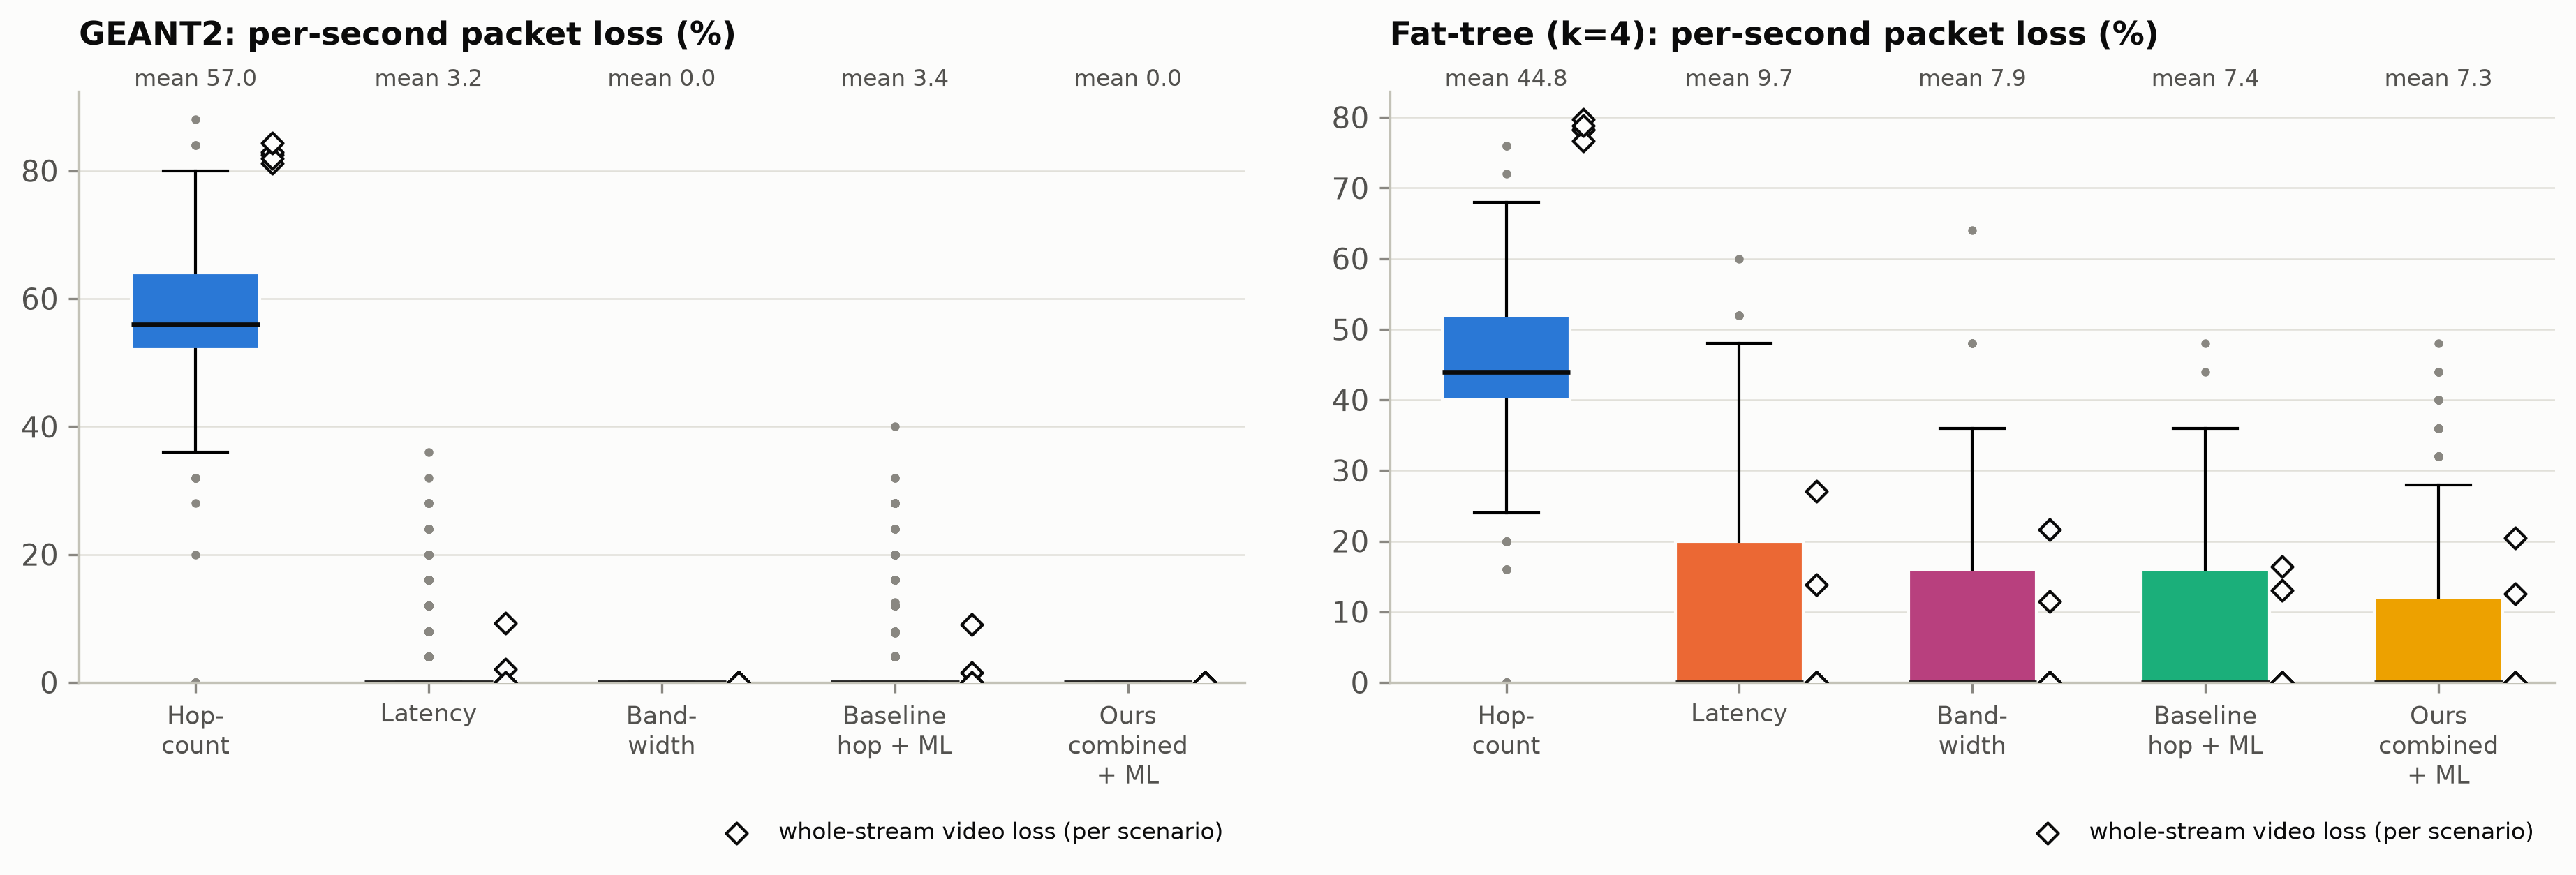
\includegraphics[width=0.49\textwidth]{loss_box.png}\\[2pt]
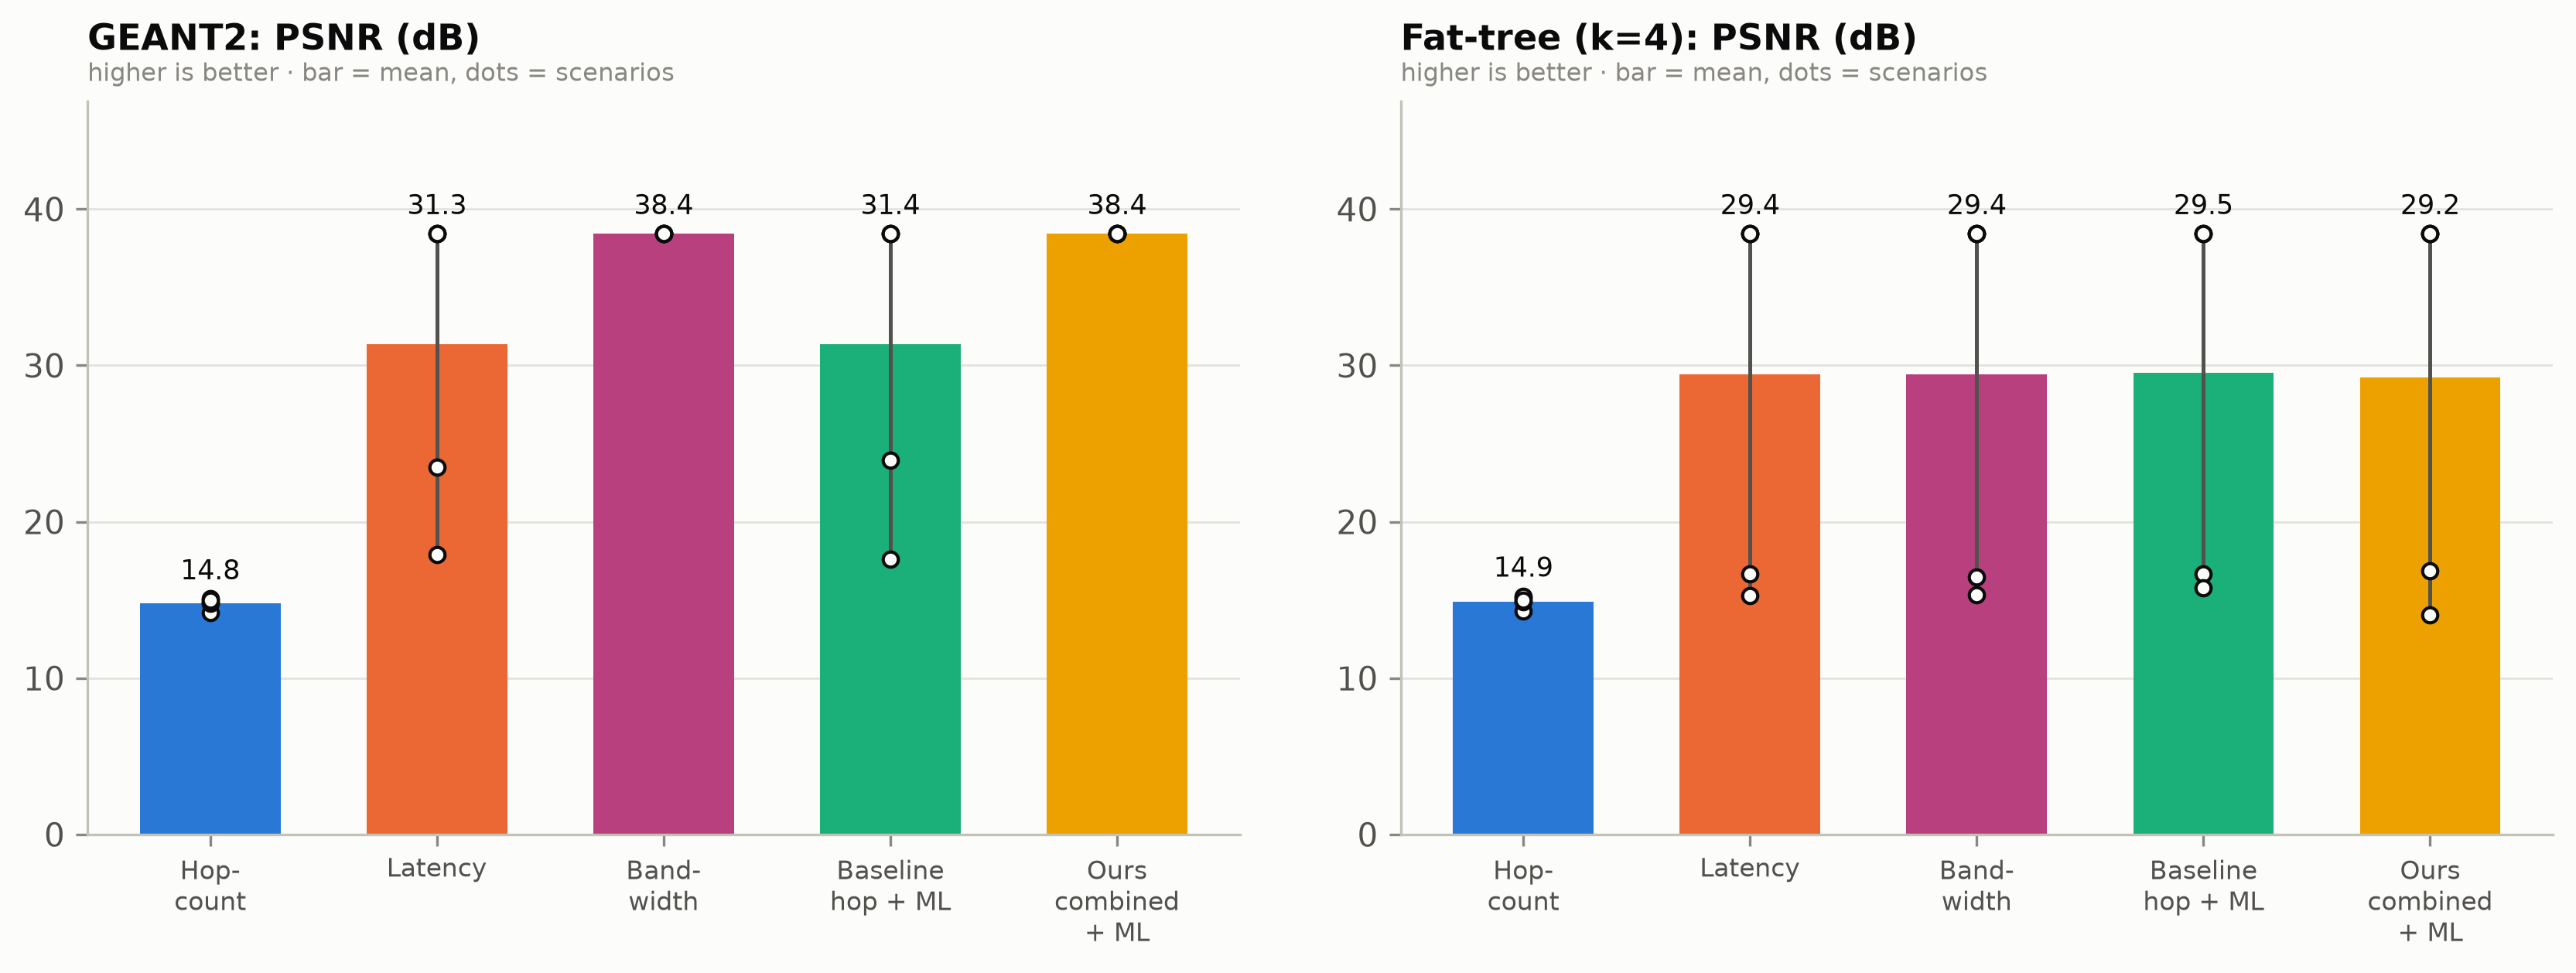
\includegraphics[width=0.49\textwidth]{psnr.png}\hfill
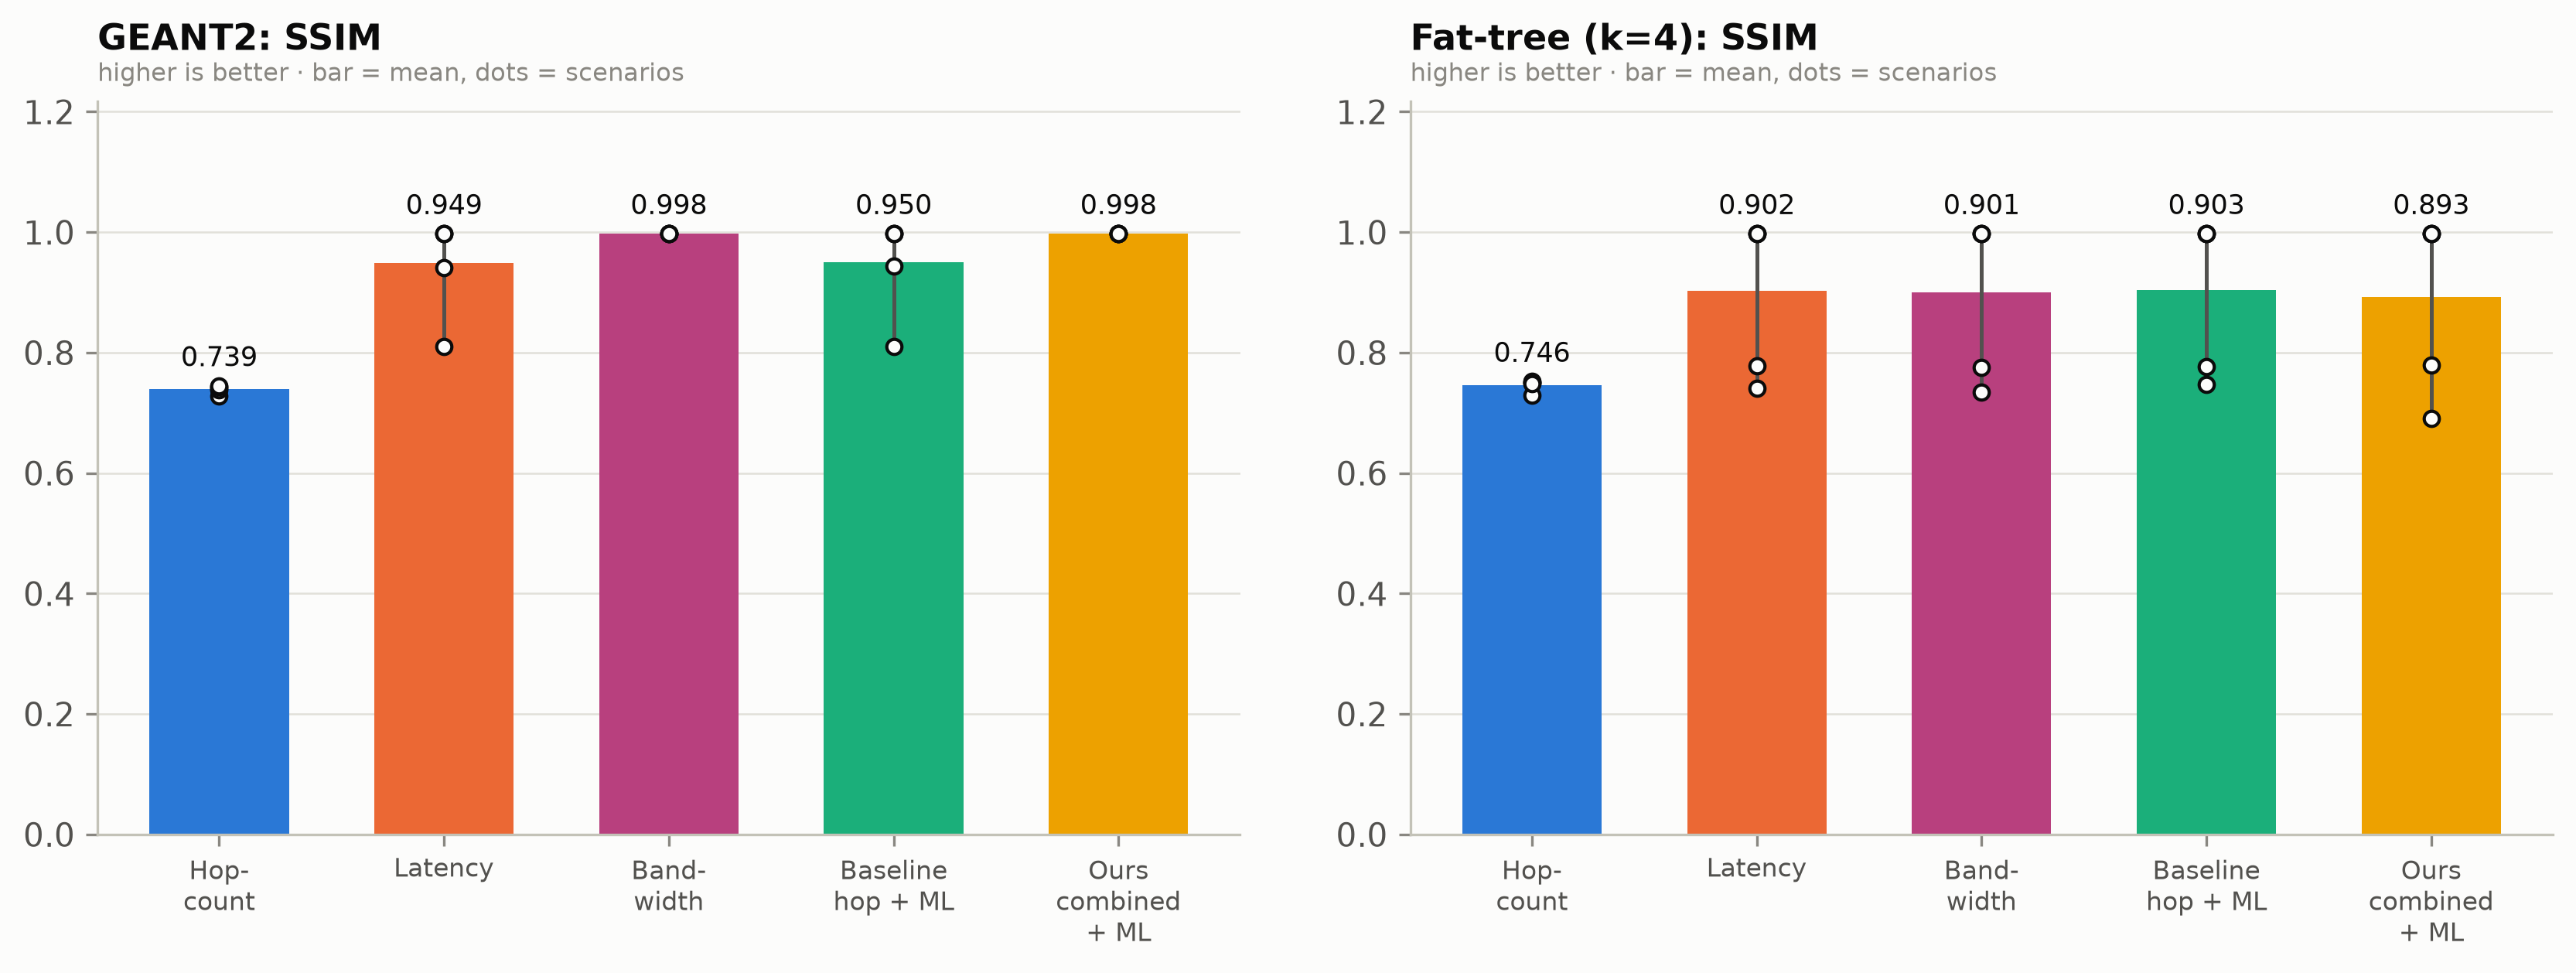
\includegraphics[width=0.49\textwidth]{ssim.png}
\caption{QoS and video quality of the five methods on GEANT2 and the fat-tree. Throughput, RTT, jitter, PSNR and
SSIM: bars are means, dots are scenarios. Packet loss: per-second probe loss pooled over scenarios (diamonds:
whole-stream video loss).}
\label{fig:qos}
\end{figure*}

\begin{figure*}[t]
\centering
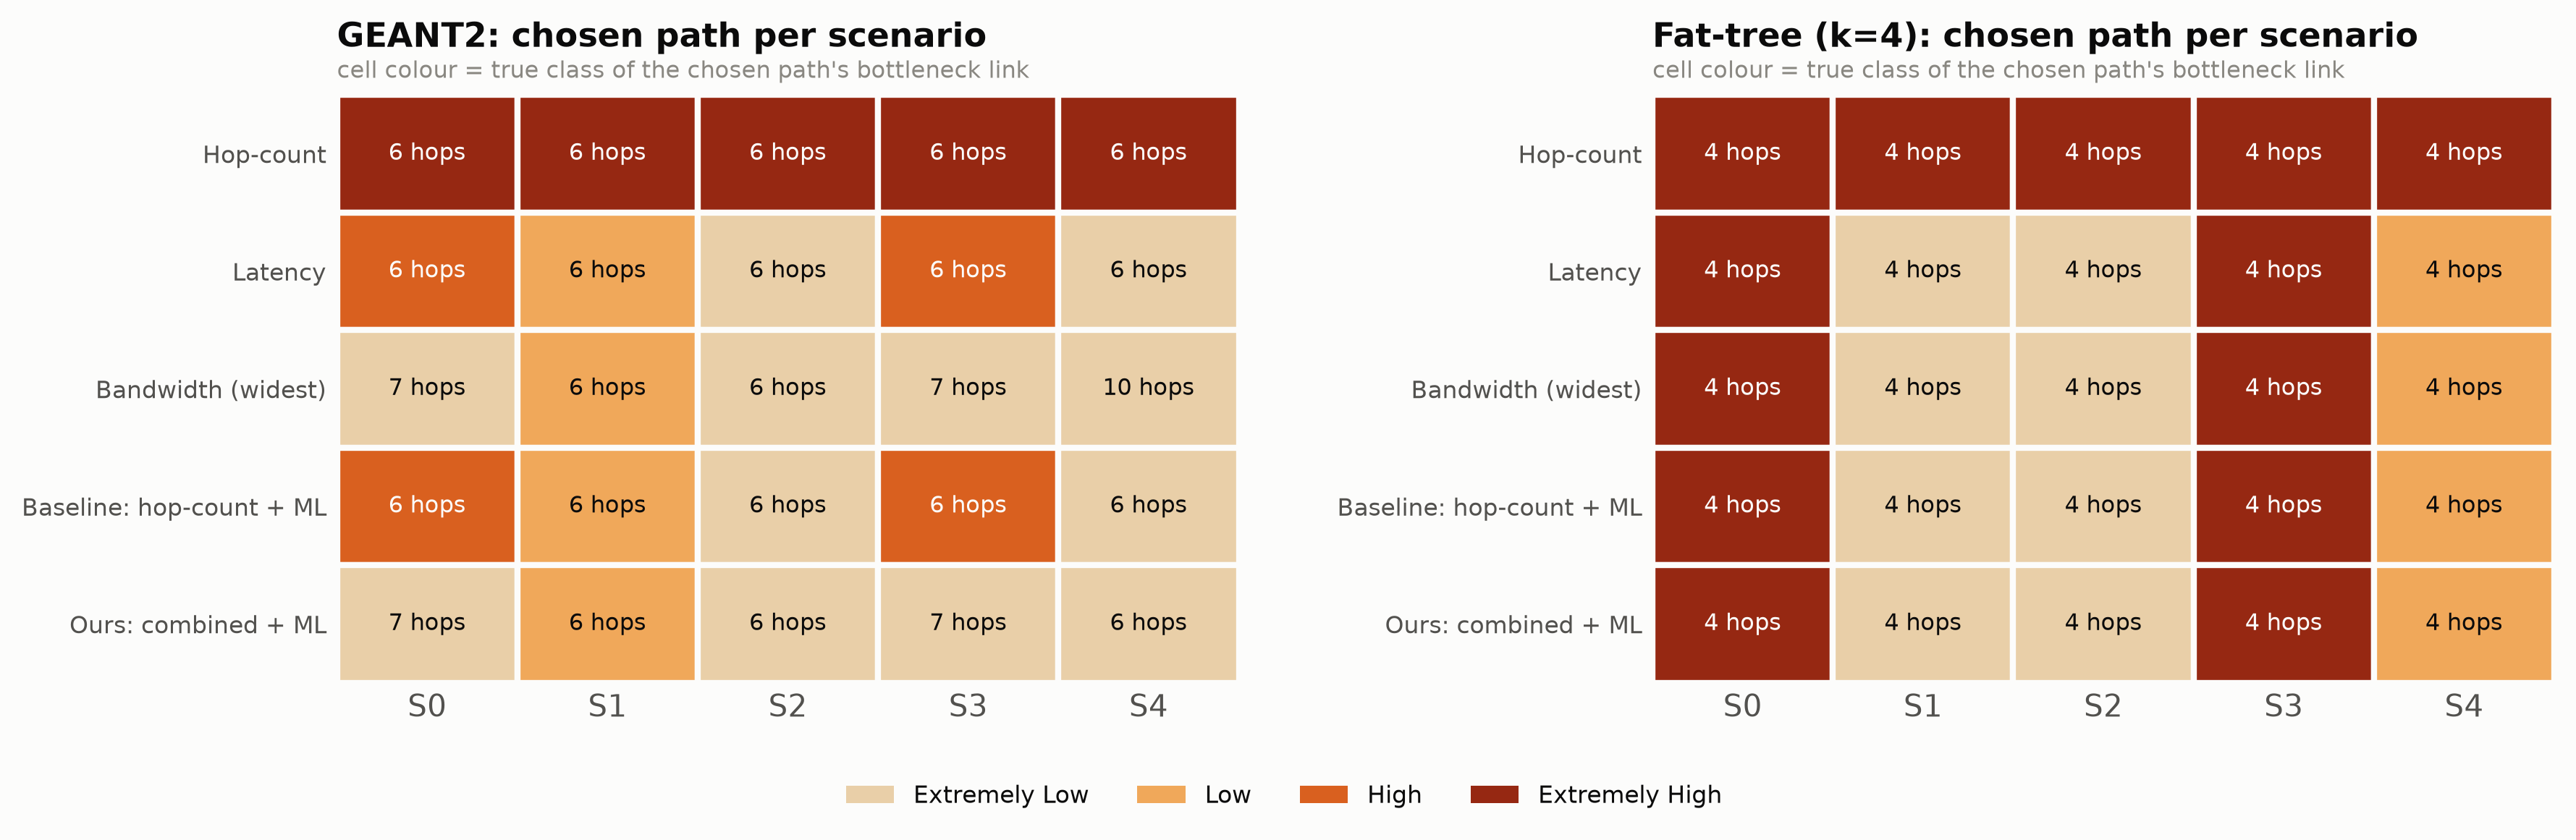
\includegraphics[width=0.9\textwidth]{paths_overview.png}
\caption{True class and length of the path each method chose in every scenario.}
\label{fig:overview}
\end{figure*}

\textit{GEANT2.} Against the baseline the proposed method removed the 2.1\,\% mean video loss (9.1\,\% in scenario~0
and 1.5\,\% in scenario~3), raised mean PSNR from 31.4 to 38.4\,dB and SSIM from 0.950 to 0.998, and cut mean RTT
from 532 to 157\,ms. Latency routing behaved like the baseline because its single lowest-delay path was the same
6-hop High path. Bandwidth routing matched the proposed method on every quality metric: the widest path is, by
construction, the one with the least-loaded bottleneck, and on GEANT2 it found the same detour. Hop-count routing,
on the forced Extremely High path, lost 82.6\,\% of the video (14.8\,dB).

\textit{Fat-tree.} All four load-aware methods reached the best reachable class in every scenario
(Table~\ref{tab:oracle}), so they share the same mean class (1.40) and similar results: 5.9--8.2\,\% loss and
29.2--29.5\,dB. The forced path s12--s4--s0--s10--s18 removes one of each endpoint's two uplinks, which eliminates
two of the four core paths and leaves only the two through s5 and s11; in scenarios 0 and 3 both of these
also crossed an Extremely High link, so every
method lost 11--27\,\% of the video and no routing choice could avoid it. In scenarios 1, 2 and 4 every load-aware
method delivered the video loss-free. The small differences between them come from run-to-run variation, not from
different decisions: in scenario~3 the baseline and the proposed method chose the same path and lost 16.4\,\% and
20.5\,\% of the video in successive runs.

\textit{Overhead.} Fig.~\ref{fig:overhead} breaks the GEANT2 decision time into its steps. Hop-count routing needs
no telemetry or probing: 2.2\,ms of path computation and 434\,ms to push the route through Floodlight's REST
interface. Both ML methods spend about 19--20\,s on telemetry, but the proposed method spent 128\,s measuring per
decision against 217\,s for the baseline, because its candidates were less congested: a probe of a congested path
waits for ping and iperf3 timeouts (iperf3 145\,s against 70\,s). Their compute plus installation time was 722\,ms
(proposed) and 764\,ms (baseline), of which route installation is about half. Stage~2 inference is one batched
call; offline it took 15.8\,ms for $K=5$ and 15.1\,ms for $K=10$, against 75.1\,ms and 157.7\,ms when the
ensemble is called once per candidate (Fig.~\ref{fig:batch}), a 4.8$\times$ and 10.4$\times$ saving. Offline,
Stage~1 took 1.1--2.2\,ms for $K=5$ with any metric.

\begin{figure*}[t]
\centering
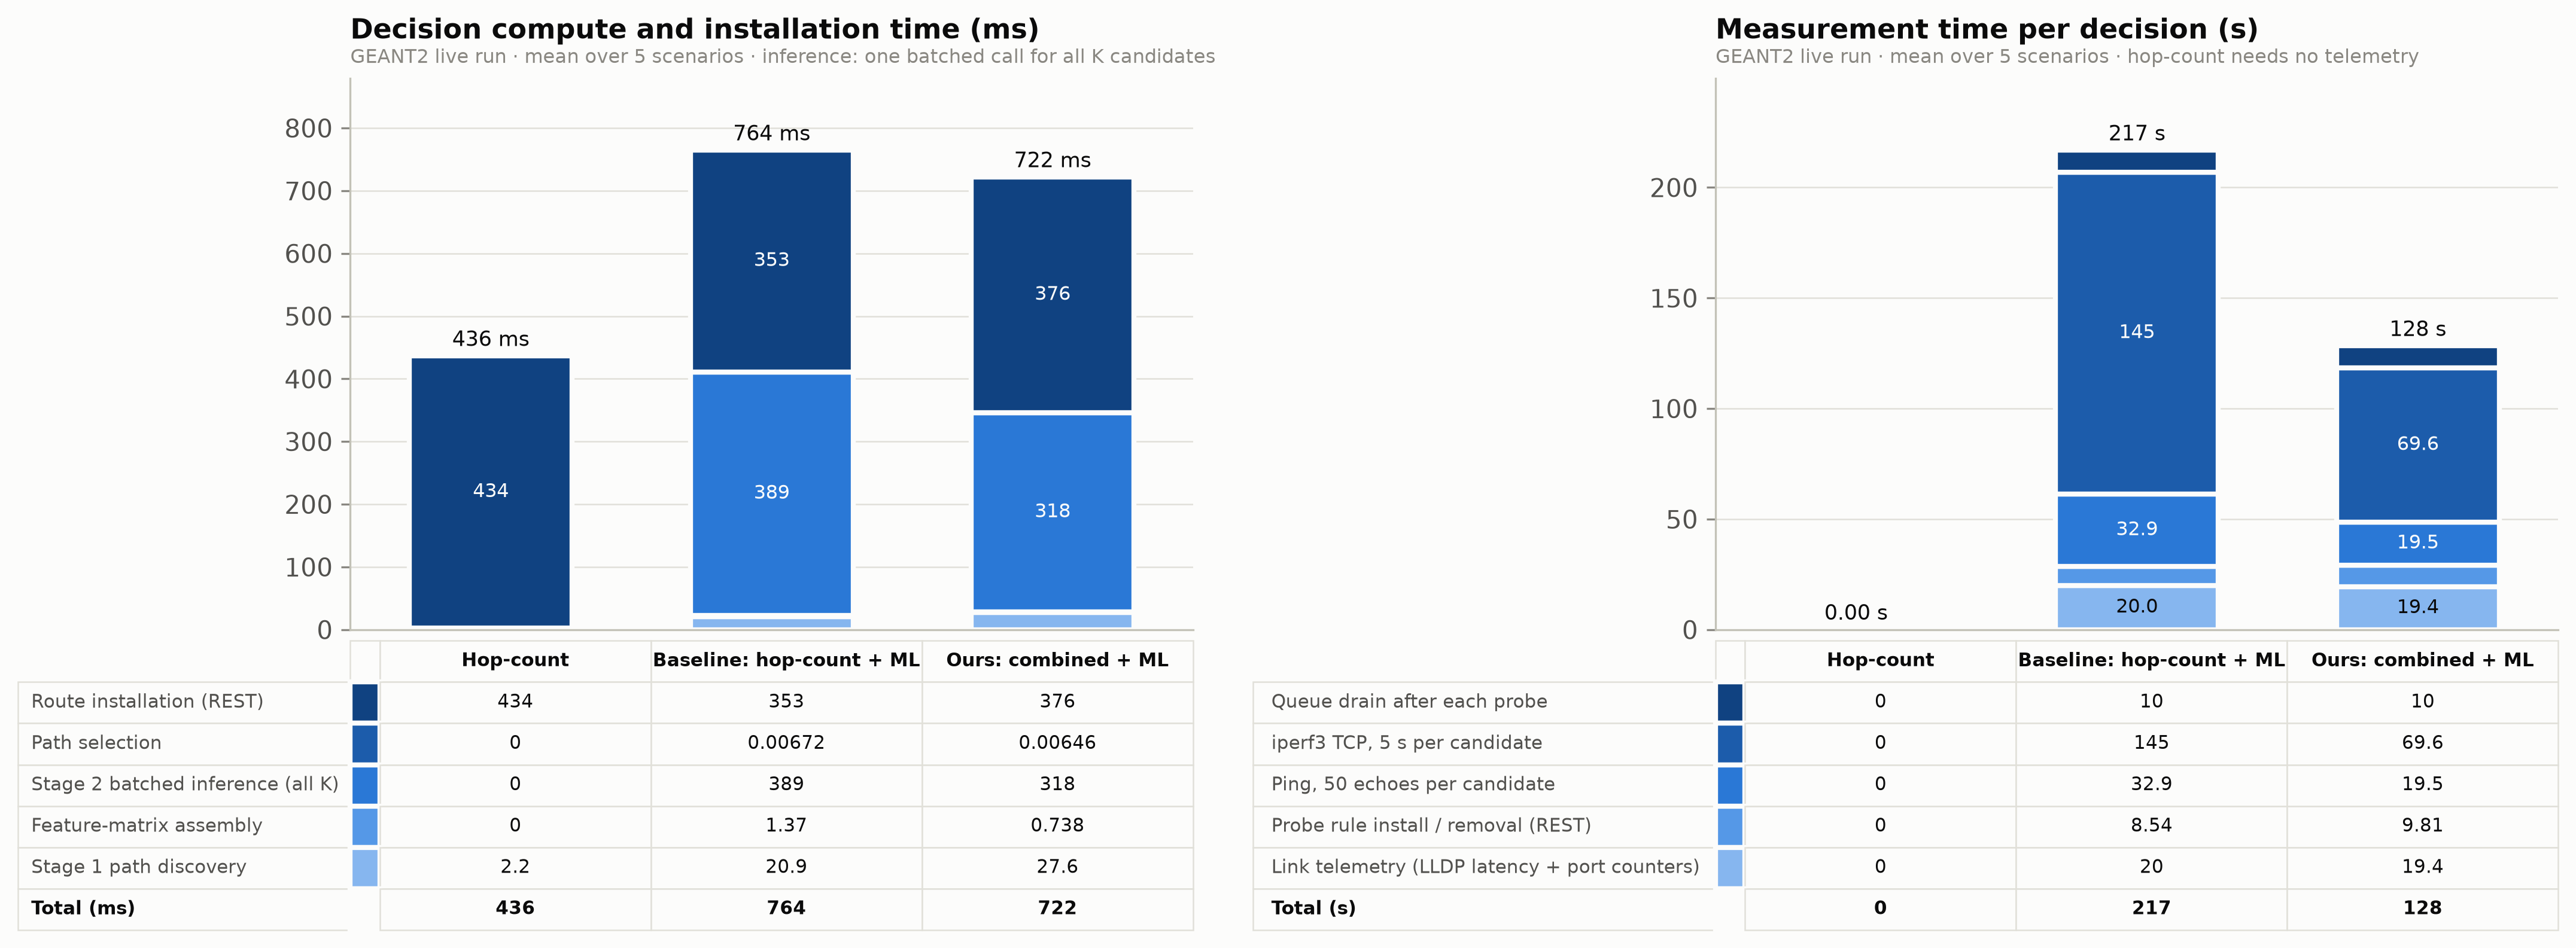
\includegraphics[width=0.94\textwidth]{overhead.png}
\caption{Per-step decision overhead on GEANT2, mean of five scenarios. Left: computation and route installation
(ms). Right: measurement (s). The table gives every step, including those too small to see.}
\label{fig:overhead}
\vspace{8pt}
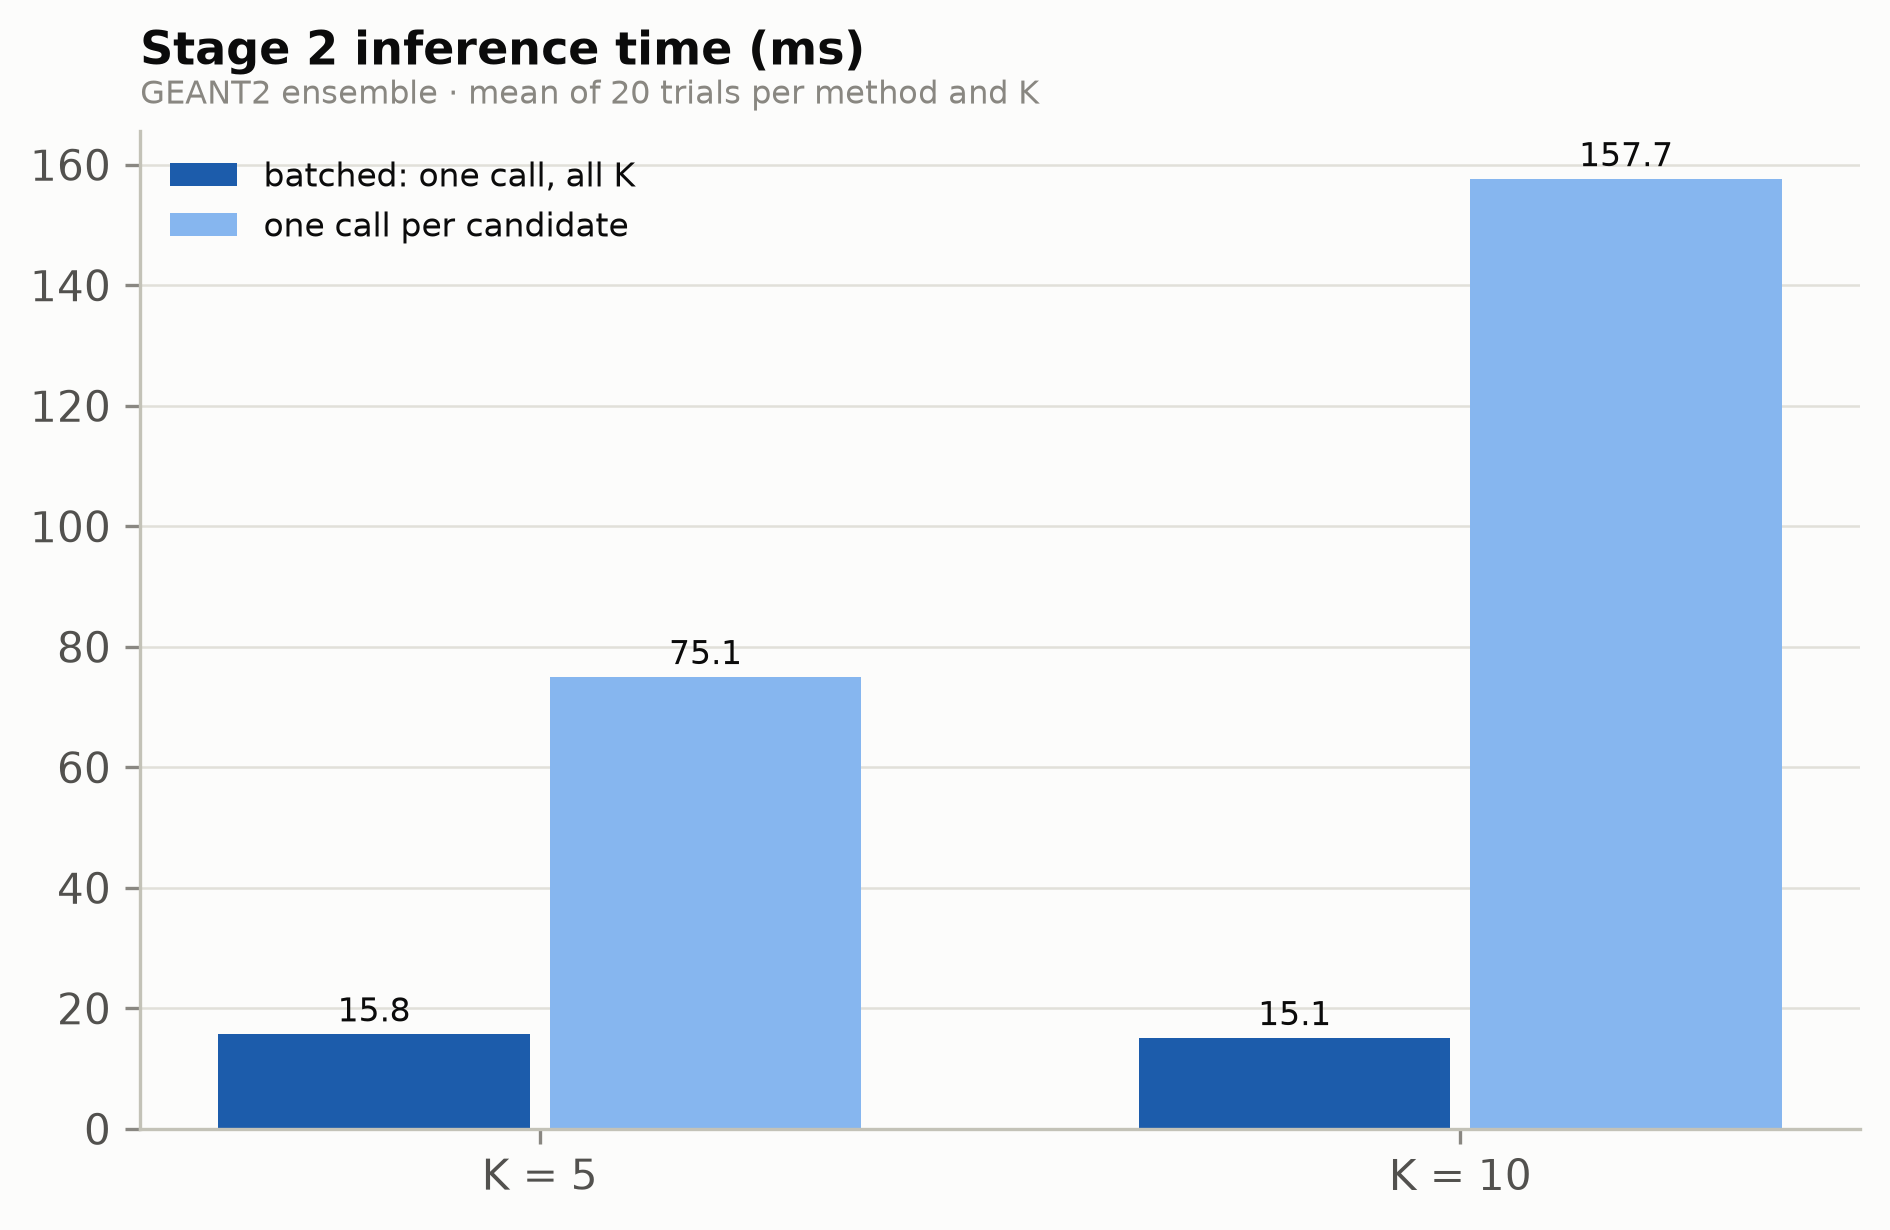
\includegraphics[width=0.46\textwidth]{batching.png}
\caption{Stage~2 inference time on GEANT2 (offline, 20 trials per Stage~1 method): one batched call for all
candidates against one call per candidate.}
\label{fig:batch}
\end{figure*}

\subsection{Discussion of Findings and Limitations}
\textit{Objectives.} Objective~1 was met: the proposed method chose the least-congested reachable path in all ten
scenarios, and on GEANT2 it did so in the two scenarios where the baseline could not. Objective~2 was met with
97.3\,\% and 98.5\,\% ensemble accuracy. Objective~3 was met on both topologies; the improvement is clear on
GEANT2 and absent on the fat-tree. Objective~4 was met: every step is timed and inference is batched.

\textit{Where the gain comes from.} The gain appears only when the best path lies outside the hop-count candidate
set. GEANT2 is meshed, so a congested region around the shortest paths can usually be bypassed by a slightly longer
detour, and the composite cost finds it. In the fat-tree every edge switch has two uplinks; once forced congestion
takes one of them, the alternatives are so few that the hop-count candidates already include the best one. A
fat-tree with more uplinks ($k>4$) or with congestion placed on core links would test this further.

\textit{Bandwidth routing as a strong baseline.} Widest-path routing matched the proposed method on both
topologies without any probing. In these scenarios a path's quality is set by its most loaded link, which the
widest path minimises directly. The ML stage adds value when telemetry is wrong or stale, which these controlled
scenarios do not exercise, and it reports a graded class that a single metric cannot.

\textit{Limitations.} (i) The results come from five scenarios per topology on a 10\,Mbit/s emulation, so small
differences, especially on the fat-tree, are within run-to-run variation. (ii) The methods run one after another
on the same scenario, so background traffic drifts slightly between them. (iii) Live inference took 318--389\,ms
against 15\,ms offline, probably because the emulation, the video and the model threads share one CPU. (iv) The
probing makes a decision take minutes, which suits long-lived flows only. (v) Each topology needs its own dataset
and model.

\FloatBarrier
% ---------------------------------------------------------------------------------------------------------
\section{Conclusion and Future Work}
This project addressed AIRSDN's reliance on hop-count candidates and binary labels for multimedia routing in SDN.
It combined a composite-cost top-5 candidate search with a four-class soft-voting ensemble that scores all
candidates in one batched call, and evaluated it with real H.264 video on GEANT2 and a $k=4$ fat-tree. On GEANT2
it chose the best reachable path in every scenario and delivered the video loss-free at 38.4\,dB PSNR and 157\,ms
RTT, against 2.1\,\% loss, 31.4\,dB and 532\,ms for the hop-count-candidate baseline, with 41\,\% less measurement
time per decision. On the fat-tree, whose sparse uplinks leave few alternatives, all load-aware methods already
reached the best path and performed alike. The main limitations are the minutes-long probing, the small number of
scenarios and the per-topology training. Future work should replace full probing with passive telemetry for
lightly loaded candidates, and test larger fat-trees and dynamic traffic that changes during the flow.

% ---------------------------------------------------------------------------------------------------------
\begin{thebibliography}{99}
\bibitem{ipek2025airsdn} A.~D. \.{I}pek \textit{et al.}, ``AIRSDN: AI based routing in software-defined networks
for multimedia traffic transmission,'' \textit{Computer Communications}, vol.~240, 2025.

\bibitem{mckeown2008openflow} N.~McKeown \textit{et al.}, ``OpenFlow: Enabling innovation in campus networks,''
\textit{ACM SIGCOMM Comput. Commun. Rev.}, vol.~38, no.~2, pp.~69--74, 2008.

\bibitem{kreutz2015sdn} D.~Kreutz, F.~M.~V. Ramos, P.~E. Ver\'issimo, C.~E. Rothenberg, S.~Azodolmolky, and
S.~Uhlig, ``Software-defined networking: A comprehensive survey,'' \textit{Proc. IEEE}, vol.~103, no.~1,
pp.~14--76, 2015.

\bibitem{karakus2017qos} M.~Karakus and A.~Durresi, ``Quality of service (QoS) in software defined networking (SDN):
A survey,'' \textit{J. Netw. Comput. Appl.}, vol.~80, pp.~200--218, 2017.

\bibitem{egilmez2012openqos} H.~E. Egilmez, S.~T. Dane, K.~T. Bagci, and A.~M. Tekalp, ``OpenQoS: An OpenFlow
controller design for multimedia delivery with end-to-end quality of service over software-defined networks,'' in
\textit{Proc. APSIPA ASC}, 2012.

\bibitem{wang1996qos} Z.~Wang and J.~Crowcroft, ``Quality-of-service routing for supporting multimedia
applications,'' \textit{IEEE J. Sel. Areas Commun.}, vol.~14, no.~7, pp.~1228--1234, 1996.

\bibitem{ma1997widest} Q.~Ma and P.~Steenkiste, ``On path selection for traffic with bandwidth guarantees,'' in
\textit{Proc. IEEE ICNP}, 1997, pp.~191--202.

\bibitem{sendra2017ai} S.~Sendra, A.~Rego, J.~Lloret, J.~M. Jimenez, and O.~Romero, ``Including artificial
intelligence in a routing protocol using software defined networks,'' in \textit{Proc. IEEE ICC Workshops}, 2017,
pp.~670--674.

\bibitem{valadarsky2017learning} A.~Valadarsky, M.~Schapira, D.~Shahaf, and A.~Tamar, ``Learning to route,'' in
\textit{Proc. ACM HotNets}, 2017, pp.~185--191.

\bibitem{mammeri2019rl} Z.~Mammeri, ``Reinforcement learning based routing in networks: Review and classification
of approaches,'' \textit{IEEE Access}, vol.~7, pp.~55916--55950, 2019.

\bibitem{rusek2020routenet} K.~Rusek, J.~Su\'arez-Varela, P.~Almasan, P.~Barlet-Ros, and A.~Cabellos-Aparicio,
``RouteNet: Leveraging graph neural networks for network modeling and optimization in SDN,'' \textit{IEEE J. Sel.
Areas Commun.}, vol.~38, no.~10, pp.~2260--2270, 2020.

\bibitem{almasan2022drlgnn} P.~Almasan, J.~Su\'arez-Varela, K.~Rusek, P.~Barlet-Ros, and A.~Cabellos-Aparicio,
``Deep reinforcement learning meets graph neural networks: Exploring a routing optimization use case,''
\textit{Computer Communications}, vol.~196, pp.~184--194, 2022.

\bibitem{yen1971kshortest} J.~Y. Yen, ``Finding the K shortest loopless paths in a network,'' \textit{Management
Science}, vol.~17, no.~11, pp.~712--716, 1971.

\bibitem{alfares2008fattree} M.~Al-Fares, A.~Loukissas, and A.~Vahdat, ``A scalable, commodity data center network
architecture,'' in \textit{Proc. ACM SIGCOMM}, 2008, pp.~63--74.

\bibitem{chen2016xgboost} T.~Chen and C.~Guestrin, ``XGBoost: A scalable tree boosting system,'' in \textit{Proc.
ACM SIGKDD}, 2016, pp.~785--794.

\bibitem{breiman2001rf} L.~Breiman, ``Random forests,'' \textit{Machine Learning}, vol.~45, no.~1, pp.~5--32, 2001.

\bibitem{friedman2001gbm} J.~H. Friedman, ``Greedy function approximation: A gradient boosting machine,''
\textit{Ann. Statist.}, vol.~29, no.~5, pp.~1189--1232, 2001.

\bibitem{cortes1995svm} C.~Cortes and V.~Vapnik, ``Support-vector networks,'' \textit{Machine Learning}, vol.~20,
no.~3, pp.~273--297, 1995.

\bibitem{platt1999probabilistic} J.~Platt, ``Probabilistic outputs for support vector machines and comparisons to
regularized likelihood methods,'' in \textit{Advances in Large Margin Classifiers}. Cambridge, MA, USA: MIT Press,
1999, pp.~61--74.

\bibitem{kuncheva2004combining} L.~I. Kuncheva, \textit{Combining Pattern Classifiers: Methods and Algorithms}.
Hoboken, NJ, USA: Wiley, 2004.

\bibitem{pedregosa2011sklearn} F.~Pedregosa \textit{et al.}, ``Scikit-learn: Machine learning in Python,''
\textit{J. Mach. Learn. Res.}, vol.~12, pp.~2825--2830, 2011.

\bibitem{lantz2010mininet} B.~Lantz, B.~Heller, and N.~McKeown, ``A network in a laptop: Rapid prototyping for
software-defined networks,'' in \textit{Proc. ACM HotNets}, 2010.

\bibitem{pfaff2015ovs} B.~Pfaff \textit{et al.}, ``The design and implementation of Open vSwitch,'' in
\textit{Proc. USENIX NSDI}, 2015, pp.~117--130.

\bibitem{floodlight} Project Floodlight, ``Floodlight OpenFlow controller.'' [Online]. Available:
\url{https://github.com/floodlight/floodlight}

\bibitem{iperf3} ESnet, ``iperf3: A TCP, UDP, and SCTP network bandwidth measurement tool.'' [Online]. Available:
\url{https://github.com/esnet/iperf}

\bibitem{ffmpeg} FFmpeg Developers, ``FFmpeg.'' [Online]. Available: \url{https://ffmpeg.org}

\bibitem{ydataprofiling} YData, ``ydata-profiling.'' [Online]. Available:
\url{https://github.com/ydataai/ydata-profiling}

\bibitem{rfc3550} H.~Schulzrinne, S.~Casner, R.~Frederick, and V.~Jacobson, ``RTP: A transport protocol for
real-time applications,'' IETF RFC 3550, 2003.

\bibitem{wang2004ssim} Z.~Wang, A.~C. Bovik, H.~R. Sheikh, and E.~P. Simoncelli, ``Image quality assessment: From
error visibility to structural similarity,'' \textit{IEEE Trans. Image Process.}, vol.~13, no.~4, pp.~600--612,
2004.
\end{thebibliography}

\end{document}
